% Options for packages loaded elsewhere
\PassOptionsToPackage{unicode}{hyperref}
\PassOptionsToPackage{hyphens}{url}
\documentclass[
]{article}
\usepackage{xcolor}
\usepackage{amsmath,amssymb}
\setcounter{secnumdepth}{-\maxdimen} % remove section numbering
\usepackage{iftex}
\ifPDFTeX
  \usepackage[T1]{fontenc}
  \usepackage[utf8]{inputenc}
  \usepackage{textcomp} % provide euro and other symbols
\else % if luatex or xetex
  \usepackage{unicode-math} % this also loads fontspec
  \defaultfontfeatures{Scale=MatchLowercase}
  \defaultfontfeatures[\rmfamily]{Ligatures=TeX,Scale=1}
\fi
\usepackage{lmodern}
\ifPDFTeX\else
  % xetex/luatex font selection
\fi
% Use upquote if available, for straight quotes in verbatim environments
\IfFileExists{upquote.sty}{\usepackage{upquote}}{}
\IfFileExists{microtype.sty}{% use microtype if available
  \usepackage[]{microtype}
  \UseMicrotypeSet[protrusion]{basicmath} % disable protrusion for tt fonts
}{}
\makeatletter
\@ifundefined{KOMAClassName}{% if non-KOMA class
  \IfFileExists{parskip.sty}{%
    \usepackage{parskip}
  }{% else
    \setlength{\parindent}{0pt}
    \setlength{\parskip}{6pt plus 2pt minus 1pt}}
}{% if KOMA class
  \KOMAoptions{parskip=half}}
\makeatother
\usepackage{color}
\usepackage{fancyvrb}
\newcommand{\VerbBar}{|}
\newcommand{\VERB}{\Verb[commandchars=\\\{\}]}
\DefineVerbatimEnvironment{Highlighting}{Verbatim}{commandchars=\\\{\}}
% Add ',fontsize=\small' for more characters per line
\newenvironment{Shaded}{}{}
\newcommand{\AlertTok}[1]{\textcolor[rgb]{1.00,0.00,0.00}{\textbf{#1}}}
\newcommand{\AnnotationTok}[1]{\textcolor[rgb]{0.38,0.63,0.69}{\textbf{\textit{#1}}}}
\newcommand{\AttributeTok}[1]{\textcolor[rgb]{0.49,0.56,0.16}{#1}}
\newcommand{\BaseNTok}[1]{\textcolor[rgb]{0.25,0.63,0.44}{#1}}
\newcommand{\BuiltInTok}[1]{\textcolor[rgb]{0.00,0.50,0.00}{#1}}
\newcommand{\CharTok}[1]{\textcolor[rgb]{0.25,0.44,0.63}{#1}}
\newcommand{\CommentTok}[1]{\textcolor[rgb]{0.38,0.63,0.69}{\textit{#1}}}
\newcommand{\CommentVarTok}[1]{\textcolor[rgb]{0.38,0.63,0.69}{\textbf{\textit{#1}}}}
\newcommand{\ConstantTok}[1]{\textcolor[rgb]{0.53,0.00,0.00}{#1}}
\newcommand{\ControlFlowTok}[1]{\textcolor[rgb]{0.00,0.44,0.13}{\textbf{#1}}}
\newcommand{\DataTypeTok}[1]{\textcolor[rgb]{0.56,0.13,0.00}{#1}}
\newcommand{\DecValTok}[1]{\textcolor[rgb]{0.25,0.63,0.44}{#1}}
\newcommand{\DocumentationTok}[1]{\textcolor[rgb]{0.73,0.13,0.13}{\textit{#1}}}
\newcommand{\ErrorTok}[1]{\textcolor[rgb]{1.00,0.00,0.00}{\textbf{#1}}}
\newcommand{\ExtensionTok}[1]{#1}
\newcommand{\FloatTok}[1]{\textcolor[rgb]{0.25,0.63,0.44}{#1}}
\newcommand{\FunctionTok}[1]{\textcolor[rgb]{0.02,0.16,0.49}{#1}}
\newcommand{\ImportTok}[1]{\textcolor[rgb]{0.00,0.50,0.00}{\textbf{#1}}}
\newcommand{\InformationTok}[1]{\textcolor[rgb]{0.38,0.63,0.69}{\textbf{\textit{#1}}}}
\newcommand{\KeywordTok}[1]{\textcolor[rgb]{0.00,0.44,0.13}{\textbf{#1}}}
\newcommand{\NormalTok}[1]{#1}
\newcommand{\OperatorTok}[1]{\textcolor[rgb]{0.40,0.40,0.40}{#1}}
\newcommand{\OtherTok}[1]{\textcolor[rgb]{0.00,0.44,0.13}{#1}}
\newcommand{\PreprocessorTok}[1]{\textcolor[rgb]{0.74,0.48,0.00}{#1}}
\newcommand{\RegionMarkerTok}[1]{#1}
\newcommand{\SpecialCharTok}[1]{\textcolor[rgb]{0.25,0.44,0.63}{#1}}
\newcommand{\SpecialStringTok}[1]{\textcolor[rgb]{0.73,0.40,0.53}{#1}}
\newcommand{\StringTok}[1]{\textcolor[rgb]{0.25,0.44,0.63}{#1}}
\newcommand{\VariableTok}[1]{\textcolor[rgb]{0.10,0.09,0.49}{#1}}
\newcommand{\VerbatimStringTok}[1]{\textcolor[rgb]{0.25,0.44,0.63}{#1}}
\newcommand{\WarningTok}[1]{\textcolor[rgb]{0.38,0.63,0.69}{\textbf{\textit{#1}}}}
\usepackage{longtable,booktabs,array}
\newcounter{none} % for unnumbered tables
\usepackage{calc} % for calculating minipage widths
% Correct order of tables after \paragraph or \subparagraph
\usepackage{etoolbox}
\makeatletter
\patchcmd\longtable{\par}{\if@noskipsec\mbox{}\fi\par}{}{}
\makeatother
% Allow footnotes in longtable head/foot
\IfFileExists{footnotehyper.sty}{\usepackage{footnotehyper}}{\usepackage{footnote}}
\makesavenoteenv{longtable}
\usepackage{graphicx}
\makeatletter
\newsavebox\pandoc@box
\newcommand*\pandocbounded[1]{% scales image to fit in text height/width
  \sbox\pandoc@box{#1}%
  \Gscale@div\@tempa{\textheight}{\dimexpr\ht\pandoc@box+\dp\pandoc@box\relax}%
  \Gscale@div\@tempb{\linewidth}{\wd\pandoc@box}%
  \ifdim\@tempb\p@<\@tempa\p@\let\@tempa\@tempb\fi% select the smaller of both
  \ifdim\@tempa\p@<\p@\scalebox{\@tempa}{\usebox\pandoc@box}%
  \else\usebox{\pandoc@box}%
  \fi%
}
% Set default figure placement to htbp
\def\fps@figure{htbp}
\makeatother
\setlength{\emergencystretch}{3em} % prevent overfull lines
\providecommand{\tightlist}{%
  \setlength{\itemsep}{0pt}\setlength{\parskip}{0pt}}
\usepackage{bookmark}
\IfFileExists{xurl.sty}{\usepackage{xurl}}{} % add URL line breaks if available
\urlstyle{same}
\hypersetup{
  hidelinks,
  pdfcreator={LaTeX via pandoc}}

\author{}
\date{}

\begin{document}

\section{Testing the Tau-Core Observer Principle with Gravitational
Lensing: Theoretical Feasibility, Data Audit, and Missing Evidence-Grade
Products}\label{testing-the-tau-core-observer-principle-with-gravitational-lensing-theoretical-feasibility-data-audit-and-missing-evidence-grade-products}

\textbf{Draft date:} 2026-05-21\\
\textbf{Repository branch:}
\texttt{codex/tau-core-lensing-observer-gate}\\
\textbf{Status:} Paper 1-style manuscript draft; theoretical test
criterion established; real-data proof not yet claimed

\subsection{Abstract}\label{abstract}

The tau-core observer principle is treated here as an operational
working hypothesis, not as a completed covariant field theory. In
standard lensing language, the paper studies a restricted perturbation
of the image-level Fermat surface: an effective latent operator whose
coefficient is shared across image systems rather than absorbed into
arbitrary per-lens nuisance freedom. The working hypothesis is that a
gravitational measurement is not only a property of the source-side mass
distribution: it is also a statement about which projection channels are
accessible to the observer. Strong gravitational lensing is a natural
place to test this principle because a single background source can be
observed through several images, each with its own parity, Fermat
potential, path geometry, and measured time delay. In this paper we ask
a deliberately limited question: is it theoretically possible to turn
the tau-core observer principle into a falsifiable gravitational-lensing
test, what data have we used to stress that test, and which data
products are still missing? The proposed test observable is a shared
amplitude, \texttt{epsilon\_tau}, multiplying the channel
\texttt{T2\_parity\_abs\_fermat}: a parity-weighted, absolute-Fermat
term that must be common across lenses and must remain distinguishable
from ordinary lens-model nuisance freedom.

We make three contributions. First, we define the necessary proof gate:
a no-T2 baseline must reproduce a published time-delay distance or null
posterior from evidence-grade image/model products before any tau-core
perturbation is allowed. Second, we show that the proposed T2 channel is
mathematically identifiable in controlled synthetic lensing experiments.
In a 28-lens hierarchical run with 224 position-constraint rows, an
injected \texttt{epsilon\_tau=0.05} is recovered as
\texttt{epsilon\_hat=0.0499193089}; blind and cached stress tests retain
the active T2 branch under core nuisance perturbations. Third, we close
a static-lens control branch using HFF cluster morphology controls.
These controls do not prove T2, but they show that the workflow does not
automatically manufacture tau-like signals in systems without a
time-delay posterior.

The present paper does not claim that the observer principle has been
proven in real lensing data. Instead, it establishes the theoretical
test pathway and the current data gap. A no-contact public-product audit
found no target with enough public image/model product depth to support
the required no-T2 reproduction gate. HE0435-1223 public imaging can be
ingested, but the public-only PSF/model route fails validation;
additional probes of RXJ1131-1231, WFI2033-4723, WGD2038-4008, and DES
J0408-5354 remain product-blocked. The result is therefore a
feasibility-and-reproducibility paper: the lensing test is well-defined
and stress-tested, but the evidence-grade public products needed for a
real-data proof are still missing.

\subsection{Author and AI-Assistance
Statement}\label{author-and-ai-assistance-statement}

This manuscript is an auditable methodological draft. The originating
author is an independent researcher and does not claim institutional
expertise in gravitational lensing, cosmography, or modified gravity.
The hypothesis, test priorities, and research direction originated from
the author and were developed with AI assistance into scripts, tables,
summaries, and prose. AI assistance is not peer review or expert
validation. The work should be evaluated by reproducibility,
conservative claim boundaries, source traceability, and independent
expert audit.

\subsection{1. Introduction: The Tau-Core Observer
Principle}\label{introduction-the-tau-core-observer-principle}

The tau-core observer principle begins from a simple measurement
distinction. In a gravitational system there is a physical source, such
as a galaxy, cluster, or lensing mass distribution. But an observer
never measures the source in itself. The observer measures light paths,
arrival times, image positions, frequency shifts, projected shapes, and
other accessible channels. The tau-core idea is that some gravitational
residuals may live not in a hidden mass component alone, and not in a
source-only modification alone, but in the mapping between source
geometry and observer-accessible projections.

In this language, \texttt{tau} is not introduced as an extra directly
observed clock that can simply be read off from data. In the present
paper, \texttt{tau} is treated as an operational latent projection
coordinate: no claim is made here that it is a covariant field, a
gauge-invariant degree of freedom, or a completed dynamical sector. The
operational question is therefore not ``can we see tau directly?'' but:

\begin{Shaded}
\begin{Highlighting}[]
\NormalTok{Can we find an observer{-}accessible channel whose geometry requires a shared}
\NormalTok{tau{-}like projection amplitude, after ordinary source/lens nuisance freedom has}
\NormalTok{been controlled?}
\end{Highlighting}
\end{Shaded}

This is why gravitational lensing is attractive. A lens does not give
one measurement of one source. It gives multiple images of the same
source through different light paths. In a time-delay lens these paths
have different arrival times and different Fermat-potential structure.
In a quad lens they also have a rich image-parity structure. Thus, a
lens is almost a natural interferometer for observer-projection ideas:
several observed channels constrain one underlying source-lens
configuration.

The tau-core observer principle would become physically meaningful in
lensing only if it predicts a constrained cross-image or cross-lens
structure. If every lens were allowed to choose its own arbitrary
correction, the idea would be empty. The test must therefore look for a
shared amplitude, common across lenses or image systems, attached to a
geometrically defined channel.

In this paper the candidate channel is:

\begin{Shaded}
\begin{Highlighting}[]
\NormalTok{T2\_parity\_abs\_fermat}
\end{Highlighting}
\end{Shaded}

It combines three ingredients that are natural in time-delay lensing:

\begin{enumerate}
\def\labelenumi{\arabic{enumi}.}
\tightlist
\item
  image parity;
\item
  Fermat-potential differences;
\item
  relative time-delay structure.
\end{enumerate}

The associated amplitude is:

\begin{Shaded}
\begin{Highlighting}[]
\NormalTok{epsilon\_tau}
\end{Highlighting}
\end{Shaded}

The goal of the present paper is not to claim that \texttt{epsilon\_tau}
has been measured. The goal is narrower and, at this stage, more
defensible:

\begin{Shaded}
\begin{Highlighting}[]
\NormalTok{1. formulate the lensing test implied by the observer principle;}
\NormalTok{2. show that the test is identifiable in synthetic lensing systems;}
\NormalTok{3. show that static controls do not automatically generate false positives;}
\NormalTok{4. audit which public data products were actually tested;}
\NormalTok{5. state precisely which evidence{-}grade products are still missing.}
\end{Highlighting}
\end{Shaded}

With that framing, the paper is a theoretical feasibility and
data-readiness study for a future proof, not a proof claim itself.

\begin{figure}
\centering
\pandocbounded{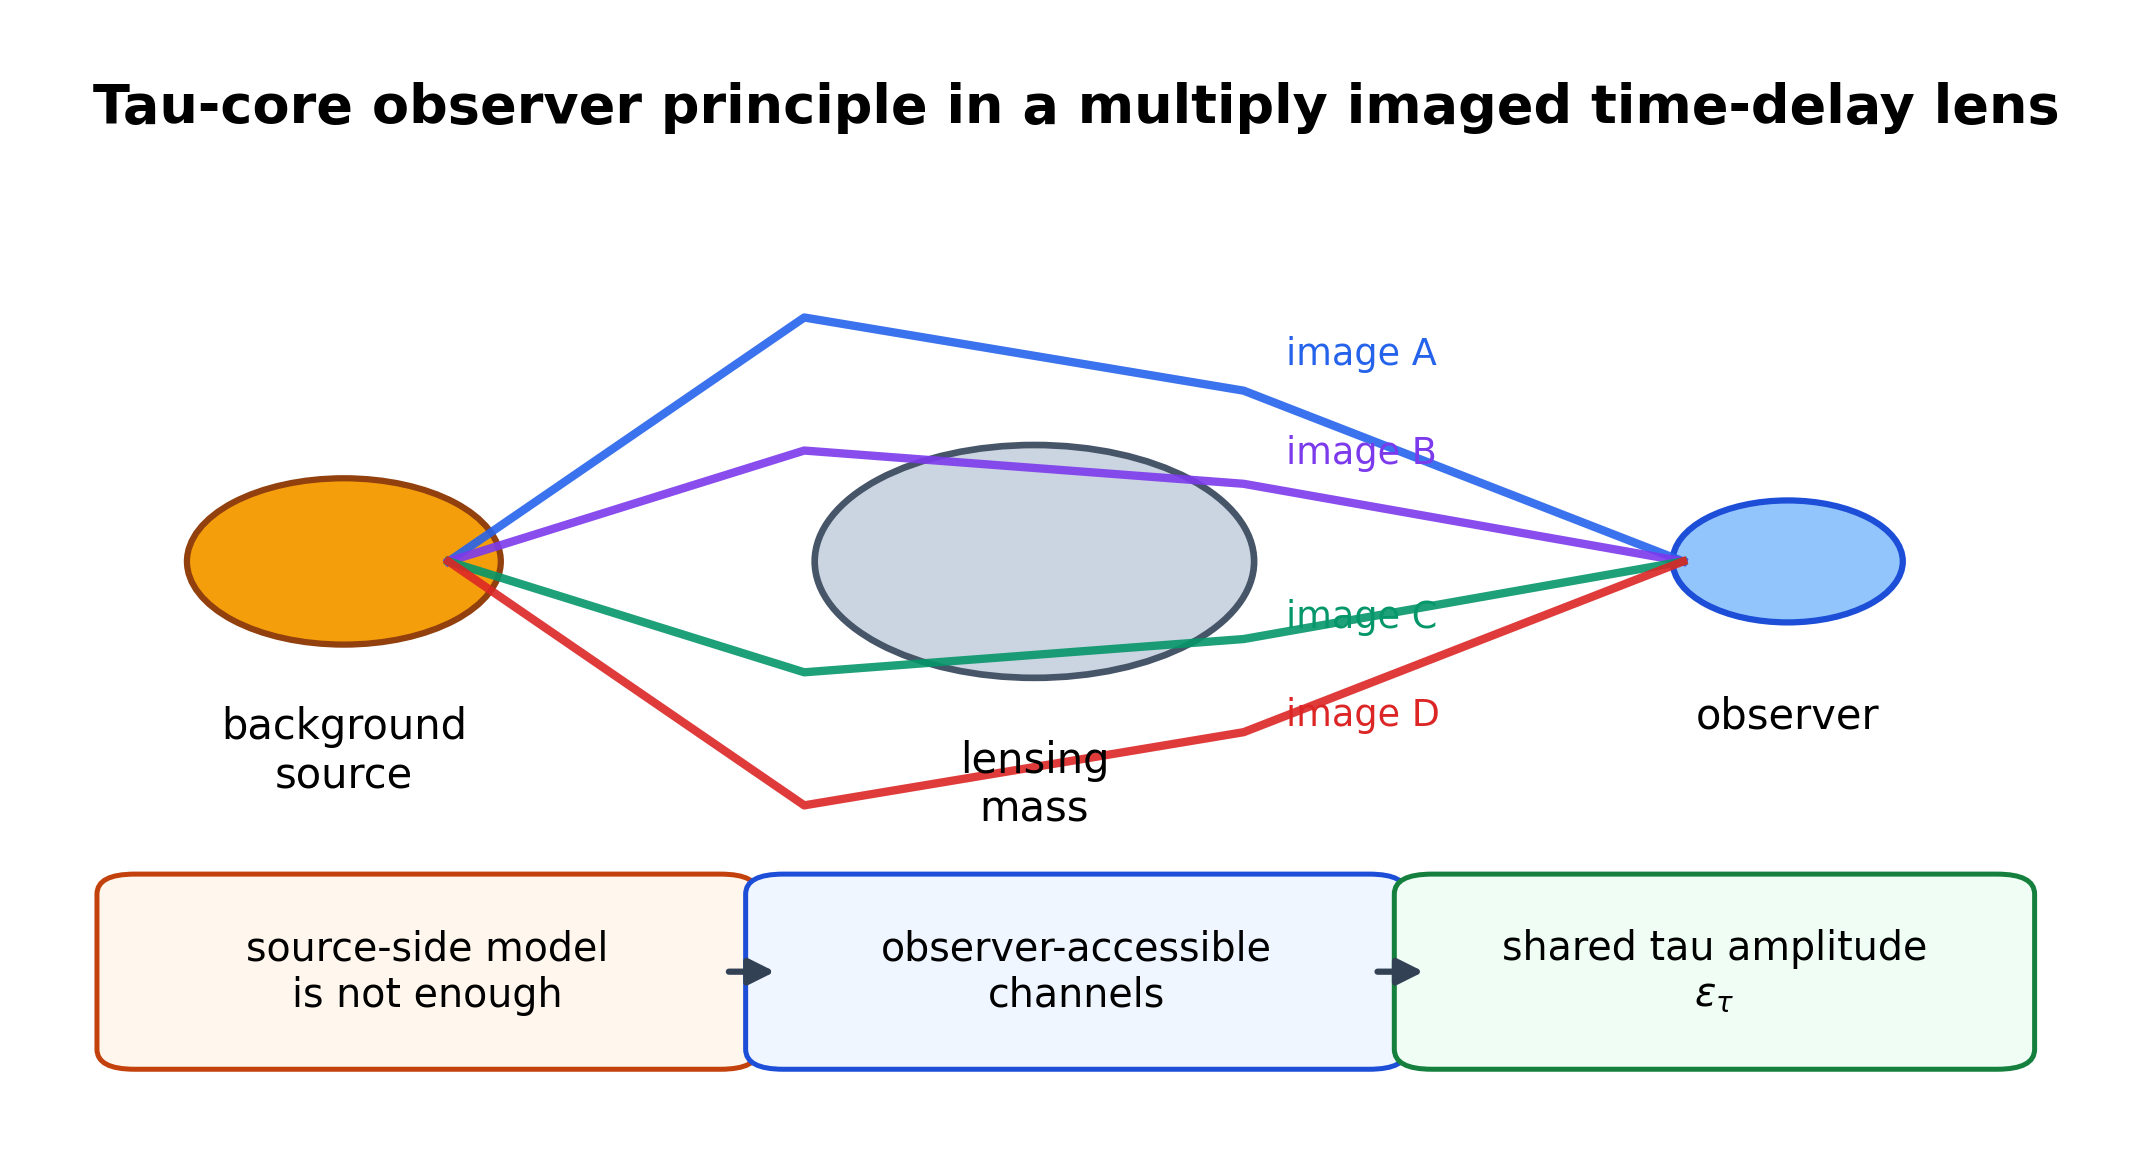
\includegraphics[keepaspectratio,alt={Figure 1. Schematic of the tau-core observer principle in a multiply imaged time-delay lens. The same background source reaches the observer through several image channels, making parity, Fermat structure, and time delays observer-accessible probes rather than source-only quantities.}]{figures/fig01_observer_principle_lensing_schematic.png}}
\caption{Figure 1. Schematic of the tau-core observer principle in a
multiply imaged time-delay lens. The same background source reaches the
observer through several image channels, making parity, Fermat
structure, and time delays observer-accessible probes rather than
source-only quantities.}
\end{figure}

\subsection{2. Toward a Physical Theory: Minimal Effective
Formulation}\label{toward-a-physical-theory-minimal-effective-formulation}

The largest weakness of the present theory is also the reason this paper
is framed as a proof-gate manuscript rather than as a modified-gravity
discovery paper. The tau-core observer principle is not yet supplied
with a complete physical definition. However, the idea can be made more
precise than a philosophical statement. This section separates three
levels. Level 0 is the measurement principle; Level 1 is the
phenomenological tau-lensing model used in this paper; Level 2 is a
complete covariant tau-core gravitational theory.

The present paper works at Level 1. It uses Level 0 as motivation and
treats Level 2 as an open theory-completion problem.

\subsubsection{2.1 Measurement Principle}\label{measurement-principle}

The measurement principle is that an observer does not access the
gravitational source directly. The observer accesses a finite set of
projection channels generated by null geodesics, arrival-time surfaces,
image parities, redshifts, and detector conventions.

The tau-core claim is that some residual structure may be attached to
this observer-accessible projection map rather than to a new source-side
mass component alone. In other words, a successful model must not merely
change the mass distribution; it must predict a constrained correction
to the map between the source-lens geometry and the observed channels.

This principle is still broad. It becomes physical only after we specify
what object carries the correction, how it transforms, how it couples to
light or to the lensing potential, and how the GR limit is recovered.

\subsubsection{2.2 Relational Observable
Ansatz}\label{relational-observable-ansatz}

The minimal phenomenological ansatz used here is not a full field
theory, but it identifies the object that a future field theory would
have to reproduce. We introduce a latent relational projection variable:

\[
\tau(x;u).
\]

The notation is deliberately conservative. The paper does not decide
whether \texttt{tau} is a scalar field, foliation variable, hidden
clock, boundary degree of freedom, information variable, or gauge
artifact. It treats \texttt{tau(x;\ u)} as a relational observable
ansatz: \texttt{x} labels the spacetime point or lens-plane location
used by the model, while \texttt{u} labels the convention by which an
observer-accessible projection is constructed.

The symbol \texttt{u} should not be read as a new preferred cosmic
frame. It is a bookkeeping label for a gauge-fixed observer
construction, analogous in spirit to choosing a tetrad, screen basis,
source-plane convention, reference image, or detector frame before
reporting lensing observables. A completed covariant theory would have
to show how this construction transforms when the observer description
is changed and which combinations are invariant. The present paper uses
\texttt{u} only to mark that the proposed residual is relational rather
than source-only.

This avoids the strongest premature interpretation. We are not
postulating a Lorentz-violating aether field, a universal foliation, or
a directly observable hidden clock. Those possibilities are not ruled
out by the notation, but they are not claimed here. The only object used
in the lensing test is the first-order projection of this relational
structure onto image-level Fermat and parity data.

At the effective lensing level, the paper does not require the full
function \texttt{tau(x;\ u)}. It requires only the first-order
image-channel projection:

\[
\delta \Phi_i = \epsilon_\tau T^{(2)}_i,
\qquad
T^{(2)}_i = \pi_i |\Delta \phi_i|.
\]

Here \texttt{Phi\_i} is the effective arrival-time/Fermat structure for
image \texttt{i}, \texttt{Delta\ phi\_i} is the model-derived
Fermat-potential difference relative to a reference image, and
\texttt{\textbackslash{}pi\_i} is the image parity or parity proxy. This
is the bridge between the broad observer principle and the actual data
test.

\subsubsection{2.3 Tau-Core Projection
Kernel}\label{tau-core-projection-kernel}

The older tau-core/TPG construction treated the observable correction as
a projection-window integral over a hidden or relational time
coordinate, not as a directly visible matter component. In its simplest
form, a projected observable correction has the structure

\[
\mathcal{P}[X]
=
\int_0^{T[X]} w(\tau)\,d\tau,
\]

where \(X\) is the ordinary observable that sets the depth of the
projection window. The tau-core symmetry assumption is dilation
covariance on positive \(\tau\)-space:

\[
w(\lambda\tau)\,d(\lambda\tau)
=
w(\tau)\,d\tau.
\]

Up to regularisation at the origin, this selects the scale-invariant
density \(w(\tau)\propto 1/\tau\). The regularised minimal
representative is

\[
w(\tau)=\frac{\alpha}{1+\tau}.
\]

Therefore a dimensionless projection depth \(T\) produces

\[
\mathcal{P}(T)
=
\alpha\int_0^T \frac{d\tau}{1+\tau}
=
\alpha\ln(1+T).
\]

For lensing, the natural image-level candidate for a dimensionless
projection depth is the Fermat offset normalized by a lens time-delay
scale:

\[
T_i
=
\frac{|\Delta\phi_i|}{\phi_\star}.
\]

In the small-window limit \(T_i\ll 1\),

\[
\mathcal{P}(T_i)
=
\alpha T_i
+\mathcal{O}(T_i^2)
=
\frac{\alpha}{\phi_\star}|\Delta\phi_i|
+\mathcal{O}(|\Delta\phi_i|^2).
\]

This supplies the tau-core origin of the absolute Fermat factor: it is
the leading term of a dilation-covariant projection-window integral when
the projection depth is the image's Fermat offset. The remaining
sign/orientation information cannot come from \(T_i\), because \(T_i\)
is a magnitude. The available local orientation invariant of the
arrival-time surface is the Morse parity
\(\pi_i=\operatorname{sgn}\det H_i\). Combining the tau projection
magnitude with Morse orientation gives

\[
\delta\Phi_i
=
\epsilon_\tau\,\pi_i|\Delta\phi_i|
+\mathcal{O}(\epsilon_\tau|\Delta\phi_i|^2,\epsilon_\tau^2).
\]

This is still not a complete derivation from a covariant action. It is,
however, a more specific tau-core physical route: dilation covariance
supplies the projection kernel, the Fermat offset supplies the lensing
projection depth, and Morse parity supplies the local orientation sign.

\subsubsection{2.4 Effective Action
Template}\label{effective-action-template}

A complete theory would require an action. This paper does not claim to
have one. The minimal action template that would be compatible with the
present lensing test has the schematic form:

\[
S =
S_\mathrm{GR}[g]
+ S_\mathrm{matter}[g,\psi]
+ S_\tau[g,\tau,u]
+ \epsilon_\tau S_\mathrm{coupling}[g,\tau,u,k].
\]

where \texttt{g} is the metric, \texttt{psi} denotes ordinary matter
fields, \texttt{u} is the gauge-fixed observer/projection construction,
and \texttt{k} is the photon/null direction. The coupling term must
reduce, in the weak-field thin-lens limit, to an image-channel
correction proportional to
\texttt{parity\_i\ *\ \textbar{}Delta\ phi\_i\textbar{}}.

This template does not define the dynamics. It defines a consistency
target: any future tau-core action that wants to explain the lensing T2
channel must produce the same first-order effective observable, while
also satisfying covariance, conservation, and the GR limit.

\subsubsection{2.5 Arrival-Time Functional
Route}\label{arrival-time-functional-route}

A more concrete variational route can be stated at the
lensing-functional level. In ordinary time-delay lensing, the image
branches are stationary points of an arrival-time functional. The
tau-core correction can be represented phenomenologically as an
additional branch functional:

\[
\mathcal{A}_\mathrm{eff}[\boldsymbol{\theta}]
=
\mathcal{A}_\mathrm{GR}[\boldsymbol{\theta}]
+ \epsilon_\tau \mathcal{A}_\tau[\boldsymbol{\theta};u].
\]

For the weak-field thin-lens reduction, the GR part is proportional to
the Fermat potential,

\[
\mathcal{A}_{\mathrm{GR},i}
\propto
\phi_i.
\]

The tau-core ansatz is that the correction does not add a new projected
mass component directly. Instead, it weights the observer-accessible
branch by the tau projection kernel and by the local Morse orientation
of the stationary point:

\[
\mathcal{A}_{\tau,i}
=
\pi_i\,\phi_\star\,\mathcal{P}
\!\left(
\frac{|\Delta\phi_i|}{\phi_\star}
\right).
\]

Using the dilation-covariant kernel from the previous subsection gives

\[
\mathcal{A}_{\tau,i}
=
\pi_i\,\phi_\star\,
\alpha
\ln\!\left(
1+\frac{|\Delta\phi_i|}{\phi_\star}
\right).
\]

For \(|\Delta\phi_i|/\phi_\star \ll 1\),

\[
\mathcal{A}_{\tau,i}
=
\alpha\,\pi_i|\Delta\phi_i|
+\mathcal{O}\!\left(
\pi_i\frac{|\Delta\phi_i|^2}{\phi_\star}
\right).
\]

Absorbing the dimensionless normalization into \(\epsilon_\tau\) yields
the T2 perturbation. This gives a concrete variational interpretation of
the operator: T2 is the leading branch contribution of a tau-projection
term added to the arrival-time functional.

The stationarity condition becomes

\[
\nabla_{\boldsymbol{\theta}}
\left(
\phi
+ \epsilon_\tau \pi\,\phi_\star
\mathcal{P}\!\left(\frac{|\Delta\phi|}{\phi_\star}\right)
\right)
=0.
\]

In the present paper we do not solve this modified lens equation. The
operational test uses the first-order correction evaluated on the
baseline GR/lens-model image branches. This is equivalent to a
perturbative treatment:

\[
\boldsymbol{\theta}_i
=
\boldsymbol{\theta}^{(0)}_i
+ \epsilon_\tau \boldsymbol{\theta}^{(1)}_i
+\mathcal{O}(\epsilon_\tau^2),
\]

while the current T2 design keeps only the branch-level shift in the
arrival-time/Fermat observable. A full theory would need to propagate
this correction consistently into image positions, magnifications, time
delays, and posterior lens parameters.

\subsubsection{2.6 Symmetry, Covariance, and Conservation
Requirements}\label{symmetry-covariance-and-conservation-requirements}

A physically acceptable Level-2 theory should satisfy at least the
following requirements:

{\def\LTcaptype{none} % do not increment counter
\begin{longtable}[]{@{}
  >{\raggedright\arraybackslash}p{(\linewidth - 2\tabcolsep) * \real{0.5000}}
  >{\raggedright\arraybackslash}p{(\linewidth - 2\tabcolsep) * \real{0.5000}}@{}}
\toprule\noalign{}
\begin{minipage}[b]{\linewidth}\raggedright
Requirement
\end{minipage} & \begin{minipage}[b]{\linewidth}\raggedright
Minimal condition
\end{minipage} \\
\midrule\noalign{}
\endhead
\bottomrule\noalign{}
\endlastfoot
diffeomorphism covariance & the full action must be coordinate
independent \\
observer-construction covariance & changes of gauge-fixed
observer/projection convention must have a defined transformation law \\
GR limit & all tau corrections vanish or become unobservable as
\texttt{epsilon\_tau\ -\textgreater{}\ 0} \\
conservation & modified field equations must imply a consistent
stress-energy balance \\
lensing consistency & null propagation must remain well-defined and
causal \\
no arbitrary per-lens freedom & the tau amplitude must be shared or
hierarchically constrained \\
\end{longtable}
}

In the present paper, only the last two operational requirements are
directly tested. The others are theory-completion gates.

\subsubsection{2.7 Gauge Meaning}\label{gauge-meaning}

The gauge problem is central. Fermat potentials, image labels, and
parity assignments are not raw detector counts; they are products of a
lens model. Therefore \texttt{T2\_i} cannot be treated as
gauge-invariant merely because it is computable. A defensible empirical
claim would require fixed image-label and reference-image conventions, a
reproducible lens-model posterior, parity derived from the same model
family, Fermat differences propagated through posterior uncertainty, and
stability of the T2 result under allowed reparameterizations.

Until this is done, the tau-lensing model is best read as a
gauge-controlled phenomenological perturbation, not as a fundamental
observable.

\subsubsection{2.8 What Is Still Open}\label{what-is-still-open}

The Level-2 theory remains incomplete. In particular, this paper does
not yet provide:

{\def\LTcaptype{none} % do not increment counter
\begin{longtable}[]{@{}
  >{\raggedright\arraybackslash}p{(\linewidth - 2\tabcolsep) * \real{0.5000}}
  >{\raggedright\arraybackslash}p{(\linewidth - 2\tabcolsep) * \real{0.5000}}@{}}
\toprule\noalign{}
\begin{minipage}[b]{\linewidth}\raggedright
Required theory ingredient
\end{minipage} & \begin{minipage}[b]{\linewidth}\raggedright
Present status
\end{minipage} \\
\midrule\noalign{}
\endhead
\bottomrule\noalign{}
\endlastfoot
covariant action & template only \\
field content & relational projection ansatz \texttt{tau(x;\ u)} only \\
covariance structure & required but not derived \\
defining symmetry & required but not derived \\
conservation relation or Ward identity & required but not derived \\
derivation of the GR limit & not derived; imposed operationally by
\texttt{epsilon\_tau\ -\textgreater{}\ 0} \\
gauge meaning of \texttt{tau} & partially specified as a
model-convention stability requirement \\
\end{longtable}
}

This is a hard claim boundary. At present, the protocol is intentionally
stronger than the theory. This is a feature of the paper's claim
boundary: it turns an under-specified principle into a falsifiable data
requirement instead of promoting it as a finished theory.

The minimal object defined in this paper is therefore not a new action.
It is an operational perturbation test on top of an ordinary lensing
baseline. The baseline lens model supplies image parity, Fermat
structure, and time-delay constraints; the observer-channel design
vector is \texttt{T2\_parity\_abs\_fermat}; the shared scalar amplitude
is \texttt{epsilon\_tau}; and the GR/null limit is recovered when
\(\epsilon_\tau=0\).

In this operational version, \texttt{T2\_parity\_abs\_fermat} is a
predefined design vector computed from lens-model products, and
\texttt{epsilon\_tau} is a shared scalar coefficient. The test asks
whether a single shared coefficient can account for structured residuals
after a no-T2 baseline and nuisance freedom have already been
controlled. This is not yet a derivation from first principles. It is a
falsifiable bridge between the observer principle and data.

The paper's theory-status statement is therefore: a complete tau-core
field theory is not yet supplied; the tau-lensing perturbation test is
defined only at phenomenological Level 1; and real-data evidence is
unavailable until a no-T2 reproduction is achieved.

\begin{figure}
\centering
\pandocbounded{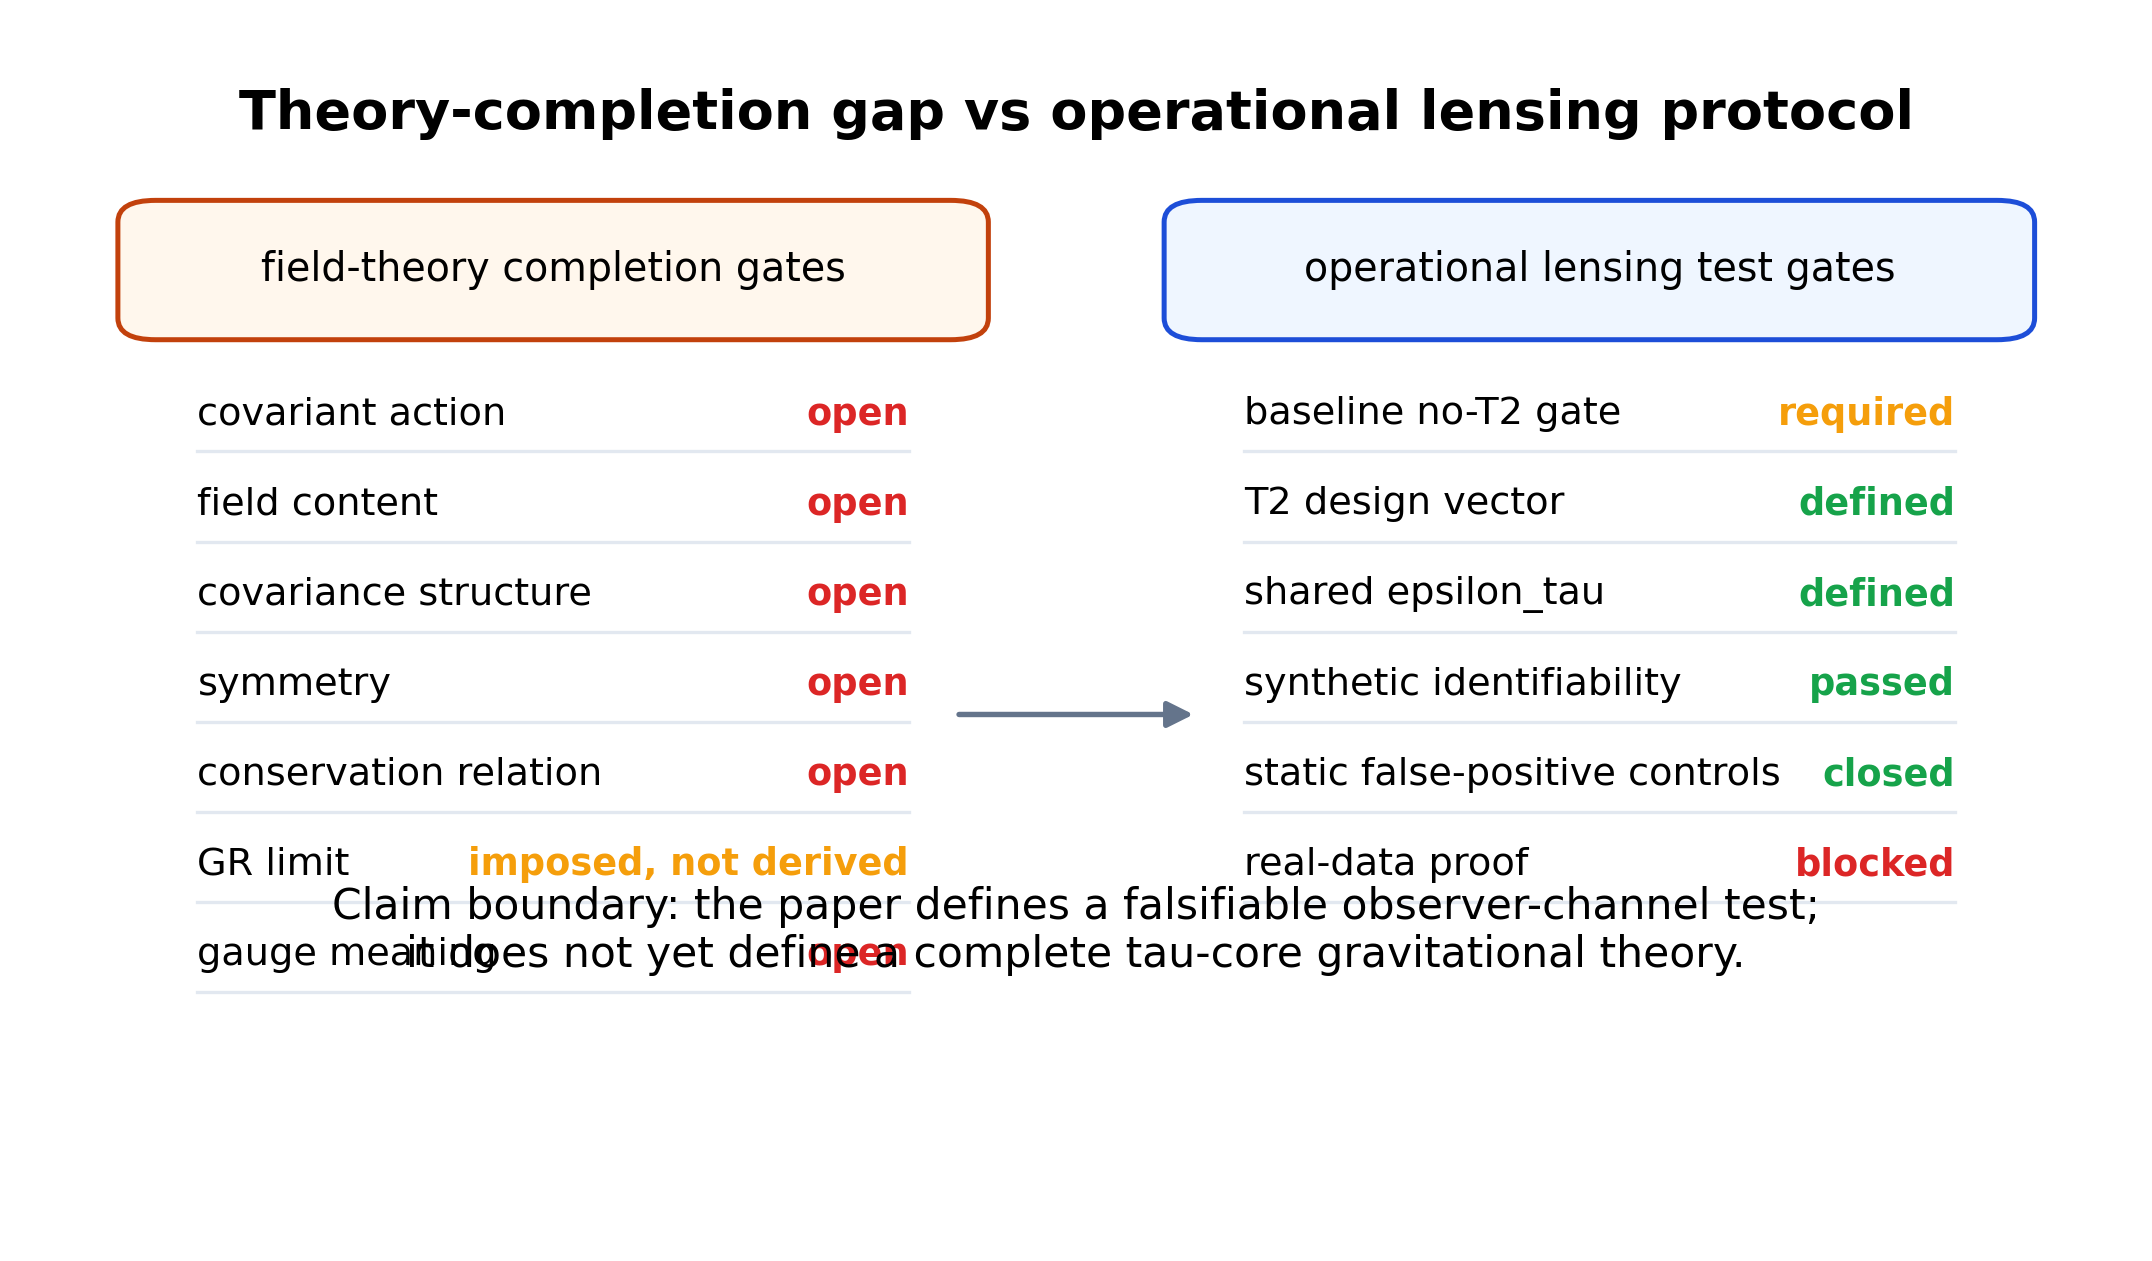
\includegraphics[keepaspectratio,alt={Figure 2. Theory-completion gap. The operational observer-gated lensing protocol is defined, while the field-theory ingredients needed for a complete physical tau-core model remain open gates.}]{figures/fig02_theory_completion_gap.png}}
\caption{Figure 2. Theory-completion gap. The operational observer-gated
lensing protocol is defined, while the field-theory ingredients needed
for a complete physical tau-core model remain open gates.}
\end{figure}

\subsection{3. Bridge to Standard Lensing and Inference
Language}\label{bridge-to-standard-lensing-and-inference-language}

The terminology used above is intentionally internal to the tau-core
program, but the statistical object is familiar. The proposed test can
be read in four standard languages.

First, in lensing perturbation language, the model is a constrained
perturbation of the Fermat surface. A conventional time-delay lensing
analysis models image positions, magnifications, and delays through a
lens potential and a Fermat potential. The tau-lensing term does not
replace that baseline. It asks whether a specific first-order residual
term, tied to parity and Fermat geometry, is favored after the baseline
model has already reproduced the published time-delay-distance or null
posterior:

\[
\Phi_i =
\Phi_i^\mathrm{GR+lens}
+ \epsilon_\tau O_i
+ N_i,
\qquad
O_i = \pi_i |\Delta \phi_i|.
\]

Second, in effective-operator language, \texttt{T2\_parity\_abs\_fermat}
is an empirical operator on image-level lens-model products. The
operator is not arbitrary: it uses quantities already present in
time-delay lensing, and it is tested against nearby controls that should
not be promoted if the effect is merely absorbing modeling freedom.
However, it is not yet theoretically inevitable. A complete dynamical
theory would need to explain why parity, absolute Fermat structure, and
a shared scalar coefficient are selected rather than another operator in
the same image-level family.

Third, in Bayesian hierarchical language, \texttt{epsilon\_tau} is a
population-level coefficient. Individual lenses may have their own
ordinary nuisance parameters, but the tau coefficient is not allowed to
float independently for every lens or image. This is the key statistical
distinction between a physical shared effect and a flexible
residual-fitting term.

\[
d_l \sim p(d_l \mid \theta_l,\eta_l,\epsilon_\tau),
\qquad
\epsilon_\tau \sim p(\epsilon_\tau),
\qquad
(\theta_l,\eta_l)\sim p_l(\theta_l,\eta_l).
\]

Fourth, in latent-variable language, \texttt{tau} is not directly
observed. It is a latent relational variable whose only allowed
appearance in this paper is through a predefined image-channel
projection. This is why compressed time-delay-distance posteriors are
insufficient: the latent projection test requires access to image
labels, parities, Fermat differences, and model uncertainties upstream
of the final cosmographic posterior.

This bridge also clarifies what the paper does not claim. It does not
claim a new mass component, a direct detection of a new field, or a
replacement for standard time-delay cosmography. It defines a
disciplined perturbation term and asks whether future evidence-grade
lensing products can falsify it.

\subsection{4. Why Lensing Is the Right Test
Bed}\label{why-lensing-is-the-right-test-bed}

The tau-core observer principle is an attempt to formalize a simple
intuition: an observer does not see a gravitational source directly; the
observer sees a projection of source geometry through accessible
measurement channels. In ordinary weak-field applications this
distinction can be hidden inside an effective potential. Strong lensing
makes the distinction sharper. A lensed quasar, for example, is observed
through multiple images of one source. These images share the same lens
but differ in parity, path geometry, Fermat potential, arrival time, and
local image constraints.

This makes time-delay lensing a natural test bed. If the observer
principle has a lensing signature, it should not appear as an arbitrary
per-lens fudge factor. It should appear as a shared, geometrically
structured amplitude that uses image-level information and survives
nuisance controls.

The central question of this paper is whether the tau-core observer
principle can be turned into a falsifiable time-delay-lensing test, and
what data products are required to run it.

Our answer is yes at the protocol level, but not yet at the real-data
proof level. We define the test criterion, test its identifiability
synthetically, audit public product availability, document the data
products actually used, and close a static-control branch.

\subsection{5. The Observer Principle in a Lensing
System}\label{the-observer-principle-in-a-lensing-system}

For a time-delay lens, a standard lens model gives image positions,
time-delay relations, and Fermat-potential differences. Let image
\texttt{i} have a parity indicator and a Fermat-potential difference
relative to a reference image. The tau-core observer principle predicts
that an admissible observer-channel correction should depend on the
multi-image geometry, not merely on a scalar distance posterior.

We therefore define the candidate T2 channel:

\begin{Shaded}
\begin{Highlighting}[]
\NormalTok{T2\_parity\_abs\_fermat}
\end{Highlighting}
\end{Shaded}

The name is intentionally operational:

\begin{itemize}
\tightlist
\item
  \texttt{parity}: the term is sensitive to image parity or a
  model-derived parity proxy;
\item
  \texttt{abs\_fermat}: the term uses absolute Fermat-potential
  structure rather than delay-only compression;
\item
  \texttt{T2}: the term is the only synthetic branch promoted as an
  active tau-core candidate in this work.
\end{itemize}

The amplitude multiplying this channel is:

\begin{Shaded}
\begin{Highlighting}[]
\NormalTok{epsilon\_tau}
\end{Highlighting}
\end{Shaded}

A crucial constraint is that \texttt{epsilon\_tau} must be shared. If
every lens, image, or exposure receives its own free amplitude, the term
is not an observer principle; it is ordinary nuisance absorption.

\subsection{6. Operator Origin and Model-Comparison
Requirement}\label{operator-origin-and-model-comparison-requirement}

The current paper does not derive \texttt{T2\_parity\_abs\_fermat} from
a dynamical principle. It motivates it as the simplest candidate
operator that uses three features special to time-delay lensing:

{\def\LTcaptype{none} % do not increment counter
\begin{longtable}[]{@{}
  >{\raggedright\arraybackslash}p{(\linewidth - 4\tabcolsep) * \real{0.3333}}
  >{\raggedright\arraybackslash}p{(\linewidth - 4\tabcolsep) * \real{0.3333}}
  >{\raggedright\arraybackslash}p{(\linewidth - 4\tabcolsep) * \real{0.3333}}@{}}
\toprule\noalign{}
\begin{minipage}[b]{\linewidth}\raggedright
Ingredient
\end{minipage} & \begin{minipage}[b]{\linewidth}\raggedright
Motivation
\end{minipage} & \begin{minipage}[b]{\linewidth}\raggedright
Remaining weakness
\end{minipage} \\
\midrule\noalign{}
\endhead
\bottomrule\noalign{}
\endlastfoot
image parity & distinguishes minima, saddles, and maxima of the
arrival-time surface & no symmetry has yet been shown to force parity
weighting \\
absolute Fermat structure & keeps sensitivity to image-level
arrival-time geometry rather than only compressed delays & no
variational derivation yet selects
\texttt{\textbar{}Delta\ phi\textbar{}} \\
shared scalar amplitude & prevents the term from becoming per-lens
residual fitting & no completed theory yet predicts a universal scalar
coefficient \\
\end{longtable}
}

Thus T2 is a first candidate in an operator family, not a final
theoretical necessity. A future dynamical tau-core theory would have to
supply at least one of the following:

\begin{enumerate}
\def\labelenumi{\arabic{enumi}.}
\tightlist
\item
  a symmetry argument that selects parity-weighted Fermat structure;
\item
  a weak-field expansion of a covariant action whose leading lensing
  correction reduces to T2;
\item
  a conservation or reciprocity relation that forbids nearby operators;
\item
  a hierarchical evidence comparison showing that T2 is favored over a
  predefined operator family after nuisance freedom is included.
\end{enumerate}

For the present paper, the conservative statement is:

\begin{Shaded}
\begin{Highlighting}[]
\NormalTok{T2 is a symmetry{-}motivated candidate operator, not a derived operator.}
\end{Highlighting}
\end{Shaded}

The necessary future comparison set should include at minimum:

{\def\LTcaptype{none} % do not increment counter
\begin{longtable}[]{@{}ll@{}}
\toprule\noalign{}
Operator & Role \\
\midrule\noalign{}
\endhead
\bottomrule\noalign{}
\endlastfoot
\(O^{(0)}_i = 0\) & standard no-tau baseline \\
\(O^{(1)}_i = \Delta \phi_i\) & ordinary signed Fermat perturbation \\
\(O^{(2)}_i = \pi_i |\Delta \phi_i|\) & current T2 candidate \\
\(O^{(3)}_i = |\Delta \phi_i|\) & parity-free absolute-Fermat control \\
\(O^{(4)}_i = \pi_i\) & parity-only control \\
\(O^{(5)}_i = L_i\) & geometric path-length proxy \\
scrambled \(O^{(2)}_i\) & label/parity/Fermat falsification control \\
\end{longtable}
}

Only an evidence comparison against this family can answer the reviewer
question ``why not another operator?''

\subsection{7. Conditional Weak-Field Derivation
Sketch}\label{conditional-weak-field-derivation-sketch}

The paper can go one step beyond naming T2 as a candidate. This section
gives a conditional derivation route. It is not yet a theorem of a
complete tau-core theory, but it states the geometrical assumptions
under which the T2 structure is the leading allowed image-channel
correction.

In the thin-lens weak-field limit, image positions are stationary points
of the Fermat potential

\[
\phi(\boldsymbol{\theta};\boldsymbol{\beta})
=
\frac{1}{2}
|\boldsymbol{\theta}-\boldsymbol{\beta}|^2
- \psi(\boldsymbol{\theta}),
\qquad
\nabla_{\boldsymbol{\theta}}\phi = 0.
\]

For image \(i\), define the Hessian

\[
H_i =
\nabla_{\boldsymbol{\theta}}\nabla_{\boldsymbol{\theta}}
\phi(\boldsymbol{\theta}_i;\boldsymbol{\beta}),
\qquad
\pi_i = \operatorname{sgn}\det H_i.
\]

The sign \(\pi_i\) is the Morse parity of the stationary point. Minima
and maxima have positive parity, while saddle images have negative
parity. Thus parity is not an additional arbitrary label; it is a
discrete invariant of the local arrival-time geometry for a fixed lens
model.

Now assume that a first-order observer-channel correction obeys four
minimal conditions:

\begin{enumerate}
\def\labelenumi{\arabic{enumi}.}
\tightlist
\item
  \textbf{Stationary-image locality:} at leading order, the correction
  is evaluated on each stationary image branch.
\item
  \textbf{Reference-shift invariance:} adding a constant to the Fermat
  potential cannot change the observable correction, so only differences
  \(\Delta\phi_i=\phi_i-\phi_\mathrm{ref}\) may enter.
\item
  \textbf{Tau-window dilation covariance:} the magnitude part of the
  correction is generated by a projection-window integral with
  \(w(\tau)=\alpha/(1+\tau)\) and \(T_i=|\Delta\phi_i|/\phi_\star\).
\item
  \textbf{Arrival-time variational origin:} the same correction can be
  represented as a branch term in an effective arrival-time functional.
\item
  \textbf{Path-reversal evenness:} the magnitude of the relational delay
  mismatch is invariant under source-observer reversal, so the leading
  scalar dependence is even in \(\Delta\phi_i\).
\item
  \textbf{Morse-orientation sensitivity:} the correction changes
  orientation across saddle versus non-saddle branches, so the only
  local discrete sign available at leading order is \(\pi_i\).
\end{enumerate}

Under these assumptions, the lowest-order scalar image-channel
correction has the form

\[
\delta\Phi_i
=
\lambda\,\pi_i\,F(|\Delta\phi_i|)
+ \mathcal{O}(\lambda^2).
\]

If the expansion is analytic in the small dimensionless Fermat offset
after normalization by the lens time-delay scale, then

\[
F(|\Delta\phi_i|)
=
c_1|\Delta\phi_i|
+ c_2|\Delta\phi_i|^2
+ \cdots .
\]

Keeping only the leading term gives

\[
\delta\Phi_i
=
\epsilon_\tau\,\pi_i|\Delta\phi_i|
+ \mathcal{O}(\epsilon_\tau |\Delta\phi_i|^2,\epsilon_\tau^2),
\]

which is precisely the T2 operator used in this paper.

This is the first concrete physics bridge in the manuscript. It says
that T2 is not selected by numerology alone: it is the leading term if
the correction is local on stationary images, invariant under Fermat
zero-point shifts, dilation-covariant in the tau-core projection window,
representable as an arrival-time functional correction, even under path
reversal in magnitude, and sensitive to Morse orientation. The open
problem is to derive these assumptions from a covariant action,
reciprocity principle, or observer-construction rule rather than
imposing them.

\subsection{8. Minimal Theorem Attempt}\label{minimal-theorem-attempt}

This section states the strongest theorem-like claim currently
available. It is not a theorem of nature; it is a conditional uniqueness
result inside the phenomenological lensing construction.

\textbf{Definitions.} Let \(\phi_i\) be the Fermat potential evaluated
on image branch \(i\), let \(\Delta\phi_i=\phi_i-\phi_\mathrm{ref}\),
and let

\[
\pi_i=\operatorname{sgn}\det H_i
\]

be the Morse parity of the image branch. Let an admissible tau-core
branch correction be a scalar map

\[
\mathcal{Q}_i
=
\mathcal{Q}(\Delta\phi_i,\pi_i;\epsilon_\tau)
\]

added perturbatively to the arrival-time/Fermat observable.

\textbf{Axioms.}

\begin{enumerate}
\def\labelenumi{\arabic{enumi}.}
\tightlist
\item
  \textbf{Branch locality.} To first order, \(\mathcal{Q}_i\) depends
  only on the stationary branch \(i\), not on an independently fitted
  per-lens amplitude.
\item
  \textbf{Fermat zero-point invariance.} \(\mathcal{Q}_i\) is invariant
  under \(\phi_i\mapsto \phi_i+C\), so it can depend on \(\Delta\phi_i\)
  but not on the absolute zero of \(\phi\).
\item
  \textbf{Tau projection depth.} The magnitude dependence enters through
  a dimensionless projection window \(T_i=|\Delta\phi_i|/\phi_\star\).
\item
  \textbf{Dilation-covariant tau weight.} The projection kernel is the
  regularized dilation-covariant density \(w(\tau)=\alpha/(1+\tau)\).
\item
  \textbf{Path-reversal evenness.} The magnitude of the correction is
  invariant under \(\Delta\phi_i\mapsto-\Delta\phi_i\).
\item
  \textbf{Morse orientation.} The only allowed first-order branch sign
  is the local Morse parity \(\pi_i\).
\item
  \textbf{Analytic small-window limit.} The correction admits an
  expansion for \(T_i\ll1\).
\end{enumerate}

\textbf{Lemma 1: magnitude term.} Axioms 3, 4, and 7 imply

\[
\mathcal{P}(T_i)
=
\alpha\ln(1+T_i)
=
\alpha T_i+\mathcal{O}(T_i^2).
\]

Thus the leading magnitude term is proportional to \(|\Delta\phi_i|\).

\textbf{Lemma 2: sign term.} Axioms 5 and 6 imply that the leading
branch sign is not \(\operatorname{sgn}(\Delta\phi_i)\), because the
magnitude is even under path reversal. The remaining local discrete
orientation supplied by the arrival-time surface is \(\pi_i\).

\textbf{Lemma 3: first-order uniqueness.} Under the above axioms, any
admissible first-order scalar correction has the form

\[
\mathcal{Q}_i
=
C\,\epsilon_\tau\,\pi_i|\Delta\phi_i|
+\mathcal{O}(\epsilon_\tau|\Delta\phi_i|^2,\epsilon_\tau^2),
\]

where \(C\) is a convention-dependent normalization absorbed into
\(\epsilon_\tau\).

\textbf{Conditional theorem.} Within this phenomenological tau-lensing
construction, the T2 operator is the unique leading first-order branch
correction satisfying branch locality, Fermat zero-point invariance,
tau-window dilation covariance, path-reversal evenness, Morse
orientation, and small-window analyticity.

The proof is conditional because the axioms are not yet derived from a
covariant action. The theorem attempt therefore upgrades T2 from a
hand-chosen operator to the leading term of a specified tau-core lensing
construction, but it does not yet prove that nature must realize that
construction.

\textbf{Proof gaps.} A complete proof would still need to derive branch
locality, path-reversal evenness, and Morse-orientation coupling from a
deeper source-observer reciprocity principle or covariant action. It
would also need to show how the modified stationarity condition
propagates into image positions, magnifications, and time-delay
posteriors without introducing uncontrolled gauge artifacts.

\subsection{9. Axiom Origin and Covariant
Closure}\label{axiom-origin-and-covariant-closure}

The conditional theorem clarifies the next physics problem: the issue is
no longer the algebraic form of T2, but the origin of the axioms. At
present the axioms have different strengths.

{\def\LTcaptype{none} % do not increment counter
\begin{longtable}[]{@{}
  >{\raggedright\arraybackslash}p{(\linewidth - 4\tabcolsep) * \real{0.3333}}
  >{\raggedright\arraybackslash}p{(\linewidth - 4\tabcolsep) * \real{0.3333}}
  >{\raggedright\arraybackslash}p{(\linewidth - 4\tabcolsep) * \real{0.3333}}@{}}
\toprule\noalign{}
\begin{minipage}[b]{\linewidth}\raggedright
Axiom
\end{minipage} & \begin{minipage}[b]{\linewidth}\raggedright
Current origin
\end{minipage} & \begin{minipage}[b]{\linewidth}\raggedright
Status
\end{minipage} \\
\midrule\noalign{}
\endhead
\bottomrule\noalign{}
\endlastfoot
Fermat zero-point invariance & standard lensing convention; only
time-delay differences are observable & physically well motivated \\
Morse orientation & standard stationary-point geometry of the Fermat
surface & geometrically well motivated \\
tau-window dilation covariance & inherited tau-core projection symmetry
& tau-core motivated, not covariantly derived \\
analytic small-window limit & ordinary effective-field/perturbative
assumption & acceptable but regime-limited \\
branch locality & perturbative image-branch assumption & plausible, not
derived \\
path-reversal evenness & candidate source-observer reciprocity principle
& open \\
Morse-orientation coupling & identification of parity as the branch
orientation sign & plausible, but needs a reciprocity or variational
theorem \\
\end{longtable}
}

This table is the current physics map. Some ingredients are standard
lensing geometry; some come from the tau-core projection kernel; some
are still imposed because the covariant completion is absent.

The missing covariant closure would need to define at least four
objects:

\begin{enumerate}
\def\labelenumi{\arabic{enumi}.}
\tightlist
\item
  \textbf{Primitive field or relational object.} A variable replacing
  the purely phenomenological \(\tau(x;u)\), together with its
  transformation law.
\item
  \textbf{Invariant observable.} A scalar or relational quantity that
  reduces to the tau projection depth \(T_i\) in the thin-lens limit.
\item
  \textbf{Conserved or constrained current.} A relation showing why the
  tau correction cannot be chosen independently on each image branch.
\item
  \textbf{Reciprocity law.} A source-observer or path-reversal statement
  explaining why the magnitude is even while the branch orientation is
  carried by \(\pi_i\).
\end{enumerate}

A schematic covariant closure would therefore have the form

\[
S[g,\psi,\tau,u]
\quad\Longrightarrow\quad
\nabla_\mu J^\mu_\tau = 0
\quad\Longrightarrow\quad
\delta\Phi_i
=
\epsilon_\tau\pi_i|\Delta\phi_i|
+\cdots
\]

in the weak-field thin-lens limit. The present paper supplies only the
last arrow conditionally. The first two arrows are the open theoretical
task.

This distinction matters because the current theorem attempt could fail
in two ways. It could fail empirically if the operator family comparison
disfavors T2. Or it could fail theoretically if a covariant completion
selects a different reciprocity law, a different projection depth, or a
different branch orientation structure.

\subsection{10. Candidate Reciprocity
Principle}\label{candidate-reciprocity-principle}

The most important missing physical ingredient is a reciprocity
principle. The candidate principle proposed here is deliberately narrow:
it is a condition on the observer-channel correction in the thin-lens
weak-field limit, not yet a full covariant theorem.

Let \(R\) denote source-observer reversal or, equivalently at this
level, orientation reversal of the image branch in the arrival-time
surface. An admissible tau-core branch correction is required to
decompose into a scalar projection depth and an orientation factor:

\[
\delta\Phi_i
=
\epsilon_\tau\,\Omega_i\,\mathcal{P}(T_i),
\]

with the transformation rules

\[
R:T_i\mapsto T_i,
\qquad
R:\mathcal{P}(T_i)\mapsto \mathcal{P}(T_i),
\qquad
R:\Omega_i\mapsto -\Omega_i.
\]

The first two conditions state why the magnitude is even: the projection
depth is a recoverability or accessibility magnitude, not an oriented
delay. In the lensing reduction this is

\[
T_i=\frac{|\Delta\phi_i|}{\phi_\star}.
\]

The third condition states that orientation must be carried by a local
orientation pseudoscalar of the image branch. For a two-dimensional
Fermat surface, the canonical local candidate is the Morse orientation

\[
\Omega_i=\pi_i=\operatorname{sgn}\det H_i.
\]

Thus the reciprocity candidate gives

\[
\delta\Phi_i
=
\epsilon_\tau\,\pi_i\,\mathcal{P}
\left(\frac{|\Delta\phi_i|}{\phi_\star}\right).
\]

Using the tau-core kernel and expanding for small \(T_i\) gives T2 at
leading order. This explains, conditionally, why the magnitude is even
and why parity carries orientation.

The same principle also suggests why the amplitude should be shared. If
\(\epsilon_\tau\) is the coupling of the projection current rather than
a per-image nuisance parameter, then different image branches sample the
same underlying tau-accessibility flux. The covariant version would
require a current or constraint such as

\[
\nabla_\mu J^\mu_\tau=0
\quad \text{or} \quad
\mathcal{C}_\tau[g,\tau,u]=0,
\]

whose thin-lens reduction leaves one shared coefficient rather than
independent branch amplitudes.

This is still a candidate principle. The missing theorem is:

\[
\text{covariant reciprocity}
\quad\Longrightarrow\quad
R:T_i\mapsto T_i,\quad
R:\Omega_i\mapsto-\Omega_i,\quad
\Omega_i=\pi_i.
\]

Until that theorem exists, path-reversal evenness, Morse-orientation
coupling, and shared amplitude are physically motivated but not derived.

\subsection{11. Reciprocity Theorem To Be
Proven}\label{reciprocity-theorem-to-be-proven}

The central theory task can now be stated more sharply. The desired
theorem is not ``T2 fits data.'' It is a covariant statement explaining
why the thin-lens observer-channel correction must decompose into an
even projection magnitude and an oriented Morse factor.

\textbf{Candidate theorem statement.} Let
\(\mathcal{O}_\tau[g,\tau,u;\gamma]\) be the detector-accessible
tau-core observable associated with a null path \(\gamma\), where \(g\)
is the metric, \(\tau\) is the relational projection object, and \(u\)
denotes the observer construction. Suppose there exists a
source-observer reversal map \(R\) such that:

\[
\mathcal{O}_\tau[R\gamma]
=
\sigma(\gamma)\,
\mathcal{O}_\tau[\gamma],
\]

where \(\sigma(\gamma)\) is an orientation character of the null branch.
The theorem needed by this program is:

\[
\sigma(\gamma_i)
\longrightarrow
\pi_i=\operatorname{sgn}\det H_i,
\qquad
|\mathcal{O}_\tau[\gamma_i]|
\longrightarrow
\mathcal{P}
\left(
\frac{|\Delta\phi_i|}{\phi_\star}
\right)
\]

in the weak-field thin-lens limit.

If this theorem were proven, then the leading branch correction would
follow:

\[
\delta\Phi_i
=
\epsilon_\tau\pi_i
\mathcal{P}
\left(
\frac{|\Delta\phi_i|}{\phi_\star}
\right)
=
\epsilon_\tau\pi_i|\Delta\phi_i|
+\cdots .
\]

The theorem requires a covariant measurable. The paper currently has
only candidates:

{\def\LTcaptype{none} % do not increment counter
\begin{longtable}[]{@{}
  >{\raggedright\arraybackslash}p{(\linewidth - 4\tabcolsep) * \real{0.3333}}
  >{\raggedright\arraybackslash}p{(\linewidth - 4\tabcolsep) * \real{0.3333}}
  >{\raggedright\arraybackslash}p{(\linewidth - 4\tabcolsep) * \real{0.3333}}@{}}
\toprule\noalign{}
\begin{minipage}[b]{\linewidth}\raggedright
Candidate measurable
\end{minipage} & \begin{minipage}[b]{\linewidth}\raggedright
Thin-lens target
\end{minipage} & \begin{minipage}[b]{\linewidth}\raggedright
Problem
\end{minipage} \\
\midrule\noalign{}
\endhead
\bottomrule\noalign{}
\endlastfoot
relational delay functional along \(\gamma\) & \(|\Delta\phi_i|\) &
needs invariant definition under observer/source exchange \\
projection-depth scalar \(T[\gamma]\) & \(|\Delta\phi_i|/\phi_\star\) &
normalization and gauge dependence must be controlled \\
tau current flux through an observer screen & shared \(\epsilon_\tau\) &
no current \(J^\mu_\tau\) is derived \\
branch-orientation character \(\sigma(\gamma)\) & \(\pi_i\) & must be
tied to Morse parity, not inserted by hand \\
\end{longtable}
}

This theorem can fail in precise ways. If no covariant scalar reduces to
\(|\Delta\phi_i|\), the magnitude part fails. If the reversal character
is not Morse parity, the parity weighting fails. If no conserved or
constrained tau current exists, the shared amplitude fails. If all three
fail, T2 remains only a phenomenological operator.

Thus the real theoretical milestone is:

\[
\boxed{
\text{covariant measurable}
+ \text{reciprocity map}
+ \text{orientation character}
\Longrightarrow
\pi_i|\Delta\phi_i|
}
\]

The present paper reaches the right-hand side conditionally. It does not
yet derive the boxed implication.

\subsection{12. Theory Companion Summary and Open
Gates}\label{theory-companion-summary-and-open-gates}

The preceding sections contain the theory needed inside this paper: the
observer-channel correction is treated as a conditional,
reciprocity-motivated weak-field candidate, not as a completed
prediction of the Tau Core parent program. The longer derivation program
now lives in the Tau Core theory hub, where it can be developed without
overloading the empirical feasibility paper.

At paper level, the relevant conditional structure is:

\[
\begin{aligned}
&\text{screen-gauge invariance}
+\text{ reciprocity-even arrival magnitude} \\
&\quad
+\text{ branch locality}
+\text{ shared observer-channel amplitude} \\
&\Longrightarrow\quad
\delta\Phi_i
=
\epsilon_\tau
\Sigma_i
\mathcal{P}(T_i^\mathrm{cov})
+O(\epsilon_\tau^2).
\end{aligned}
\]

In the weak-field thin-lens limit,

\[
\Sigma_i\to\pi_i,
\qquad
T_i^\mathrm{cov}\to\frac{|\Delta\phi_i|}{\phi_\star},
\]

so the candidate leading term becomes

\[
\delta\Phi_i
=
\epsilon_\tau
\pi_i
\mathcal{P}
\left(
\frac{|\Delta\phi_i|}{\phi_\star}
\right)
=
\epsilon_\tau\pi_i|\Delta\phi_i|
+O(\epsilon_\tau|\Delta\phi_i|^2,\epsilon_\tau^2).
\]

The detailed theory companion is the
\href{../../../tau-core-theory-main/source_material/tau_core_foundations/lensing_observer_gate_theory_module_v01.md}{Tau Core theory-hub lensing module}.
It tracks the longer proof route and the open theory gates:

{\def\LTcaptype{none} % do not increment counter
\begin{longtable}[]{@{}
  >{\raggedright\arraybackslash}p{(\linewidth - 4\tabcolsep) * \real{0.3333}}
  >{\raggedright\arraybackslash}p{(\linewidth - 4\tabcolsep) * \real{0.3333}}
  >{\raggedright\arraybackslash}p{(\linewidth - 4\tabcolsep) * \real{0.3333}}@{}}
\toprule\noalign{}
\begin{minipage}[b]{\linewidth}\raggedright
Gate
\end{minipage} & \begin{minipage}[b]{\linewidth}\raggedright
Paper status
\end{minipage} & \begin{minipage}[b]{\linewidth}\raggedright
Theory-hub role
\end{minipage} \\
\midrule\noalign{}
\endhead
\bottomrule\noalign{}
\endlastfoot
full reciprocity theorem & conditional theorem target & prove or refute
the orientation/magnitude decomposition \\
covariant measurable & candidate via Jacobi orientation and arrival-time
scalar & derive the detector-accessible invariant \\
tau-accessibility current & shared-amplitude candidate & derive
conservation or a constrained observer-channel law \\
screen interaction & controlled effective insertion & derive from
boundary variation or replace with a better coupling \\
dynamical closure / GR limit & requirements stated & derive
stress-energy, conservation, and decoupling from a parent action \\
\end{longtable}
}

This paper therefore uses the theory only to justify a falsifiable
operator family and a data protocol. It does not claim that the parent
theory has already forced the T2 operator uniquely.

\subsection{13. Missing Geometric
Necessity}\label{missing-geometric-necessity}

The strongest remaining physics gap is not statistical. It is geometric.
The paper defines an observable framework, a candidate operator family,
a conditional weak-field route, and a future inference procedure, but it
does not yet show that the T2 structure is forced by a deeper geometry.

A stronger theory would need at least one geometrical selection
mechanism:

{\def\LTcaptype{none} % do not increment counter
\begin{longtable}[]{@{}
  >{\raggedright\arraybackslash}p{(\linewidth - 2\tabcolsep) * \real{0.5000}}
  >{\raggedright\arraybackslash}p{(\linewidth - 2\tabcolsep) * \real{0.5000}}@{}}
\toprule\noalign{}
\begin{minipage}[b]{\linewidth}\raggedright
Missing mechanism
\end{minipage} & \begin{minipage}[b]{\linewidth}\raggedright
What it would need to show
\end{minipage} \\
\midrule\noalign{}
\endhead
\bottomrule\noalign{}
\endlastfoot
symmetry necessity & a transformation principle that singles out
parity-weighted Fermat structure \\
variational derivation & an action whose weak-field lensing limit
produces the T2 operator \\
reciprocity theorem & a source-observer or path-reversal identity that
requires the same correction \\
caustic/parity theorem & a result tying saddle/minimum parity structure
to the residual sign or weight \\
dynamical selection rule & a reason the shared scalar amplitude is
universal or hierarchical \\
\end{longtable}
}

At present, none of these has been derived. This means the physics
kernel is embryonic: the paper has a disciplined way to test a candidate
geometrical idea, but it does not yet contain the theorem that would
make the candidate inevitable.

The most accurate classification of the work is therefore:

\begin{Shaded}
\begin{Highlighting}[]
\NormalTok{new physics claim: not established}
\NormalTok{geometrical necessity: not derived}
\NormalTok{phenomenological test kernel: defined}
\NormalTok{falsification and inference protocol: strong}
\end{Highlighting}
\end{Shaded}

This distinction is important. A negative future test would falsify the
proposed T2 phenomenology, not every possible tau-core theory. A
positive future test would motivate a deeper geometrical derivation, but
would not by itself complete the theory.

\subsection{14. Breakthrough Roadmap}\label{breakthrough-roadmap}

The current manuscript is not the breakthrough. It is the scaffold that
states what a breakthrough would have to look like. Three next results
would change the scientific status of the program.

The primary theoretical game changer would be a weak-field derivation.
If the T2 structure emerged as the leading correction in a controlled
weak-field expansion,

\[
\Phi_i =
\Phi_i^\mathrm{GR}
+ \lambda \pi_i|\Delta\phi_i|
+ \mathcal{O}(\lambda^2),
\]

then the program would move from a phenomenological operator test to a
candidate geometrical theory. The crucial point is not merely the
appearance of \(|\Delta\phi_i|\), but the joint emergence of parity
weighting, absolute Fermat structure, and a shared amplitude.

The most attractive geometrical route to such a result may be a
reciprocity or parity theorem. A theorem of this kind would connect
source-observer exchange, path reversal, or caustic crossing structure
to the sign/weight carried by the image parity \(\pi_i\). The target
statement would have the schematic form:

\[
\mathcal{G}_\mathrm{lens}
\quad \Longrightarrow \quad
\delta \Phi_i \propto \pi_i |\Delta \phi_i|
\quad
\text{at leading order}.
\]

The first serious empirical milestone would be real-data operator
competition. The decisive comparison is not T2 versus nothing in
isolation, but T2 against the operator family
\(\{O^{(0)},\ldots,O^{(5)}\}\) after marginalizing lens-model nuisance
freedom:

\[
Z_2 > Z_m
\quad \text{for relevant controls } m \ne 2,
\]

with stability under prior sensitivity and posterior-predictive checks.

Until one of these results exists, the paper should be read as a
disciplined phenomenological and falsification framework, not as a
completed physics theory.

\subsection{15. Likelihood and Evidence
Framework}\label{likelihood-and-evidence-framework}

Because the paper uses population-level language, the future real-data
test must be stated as a likelihood problem. For lens \texttt{l} and
image-level data vector \texttt{d\_l}, let \texttt{theta\_l} denote
ordinary lens parameters and \texttt{eta\_l} denote nuisance/systematic
parameters. For an operator \texttt{O\_m}, the model is:

\[
d_l \sim
p\!\left(d_l \mid \theta_l,\eta_l,\epsilon_m,O^{(m)}\right),
\qquad
\epsilon_m \sim p(\epsilon_m),
\qquad
(\theta_l,\eta_l) \sim p(\theta_l,\eta_l).
\]

The posterior for a candidate operator is:

\[
p\!\left(
\epsilon_m,\{\theta_l\},\{\eta_l\}
\mid
\{d_l\},O^{(m)}
\right)
\propto
p(\epsilon_m)
\prod_l p(\theta_l,\eta_l)
\prod_l
p\!\left(d_l\mid\theta_l,\eta_l,\epsilon_m,O^{(m)}\right).
\]

The evidence for the operator is:

\[
Z_m =
\int
p(\epsilon_m)
\prod_l p(\theta_l,\eta_l)
\prod_l p\!\left(d_l\mid\theta_l,\eta_l,\epsilon_m,O^{(m)}\right)
\,d\epsilon_m\,d\theta_l\,d\eta_l.
\]

The relevant comparison is not simply whether \texttt{epsilon\_m} is
nonzero. It is whether the T2 operator improves predictive and
evidential performance after the Occam penalty for the shared
coefficient and after marginalizing ordinary lens-model freedom. The
no-tau comparison is:

\[
B_{20} = \frac{Z_2}{Z_0}.
\]

The operator-competition requirement is to compare \(Z_m\) across the
predefined operator family. Posterior-predictive simulations must
reproduce the residual structure without creating false positives in
controls, and the conclusion must be stable under reasonable priors on
\(\epsilon_m\) and nuisance widths.

The present paper does not compute these real-data evidences because the
required image/model products are not available in the public-only
route. It does, however, define the likelihood objects that a future
evidence-grade test must instantiate.

\subsection{16. What Would Count as a Future
Proof?}\label{what-would-count-as-a-future-proof}

We use the word proof operationally, not metaphysically. A
gravitational-lensing proof of the observer principle would require all
of the following:

\begin{enumerate}
\def\labelenumi{\arabic{enumi}.}
\tightlist
\item
  A public or auditable image/model product chain for one or more
  time-delay lenses.
\item
  A no-T2 model that reproduces a published Ddt or null posterior within
  a preregistered tolerance.
\item
  Image labels, positions, parity or parity-computable models, relative
  delays, and Fermat-potential differences.
\item
  A T2 perturbation with one shared \texttt{epsilon\_tau}, not
  per-object amplitudes.
\item
  A likelihood-level posterior for \texttt{epsilon\_tau}, with nuisance
  parameters marginalized.
\item
  Evidence or predictive improvement over the no-tau baseline and over
  nearby operator controls.
\item
  Prior-sensitivity and posterior-predictive checks.
\item
  A null result when the T2 channel is removed or scrambled.
\end{enumerate}

The proof condition can be summarized as:

In words, a future proof would require a successful standard no-T2
reproduction, a statistically identified shared \texttt{epsilon\_tau},
and survival under nuisance, scrambling, and false-positive controls.

This paper satisfies the last three items only in synthetic/control
form. It does not satisfy the first two real-data requirements.

\begin{figure}
\centering
\pandocbounded{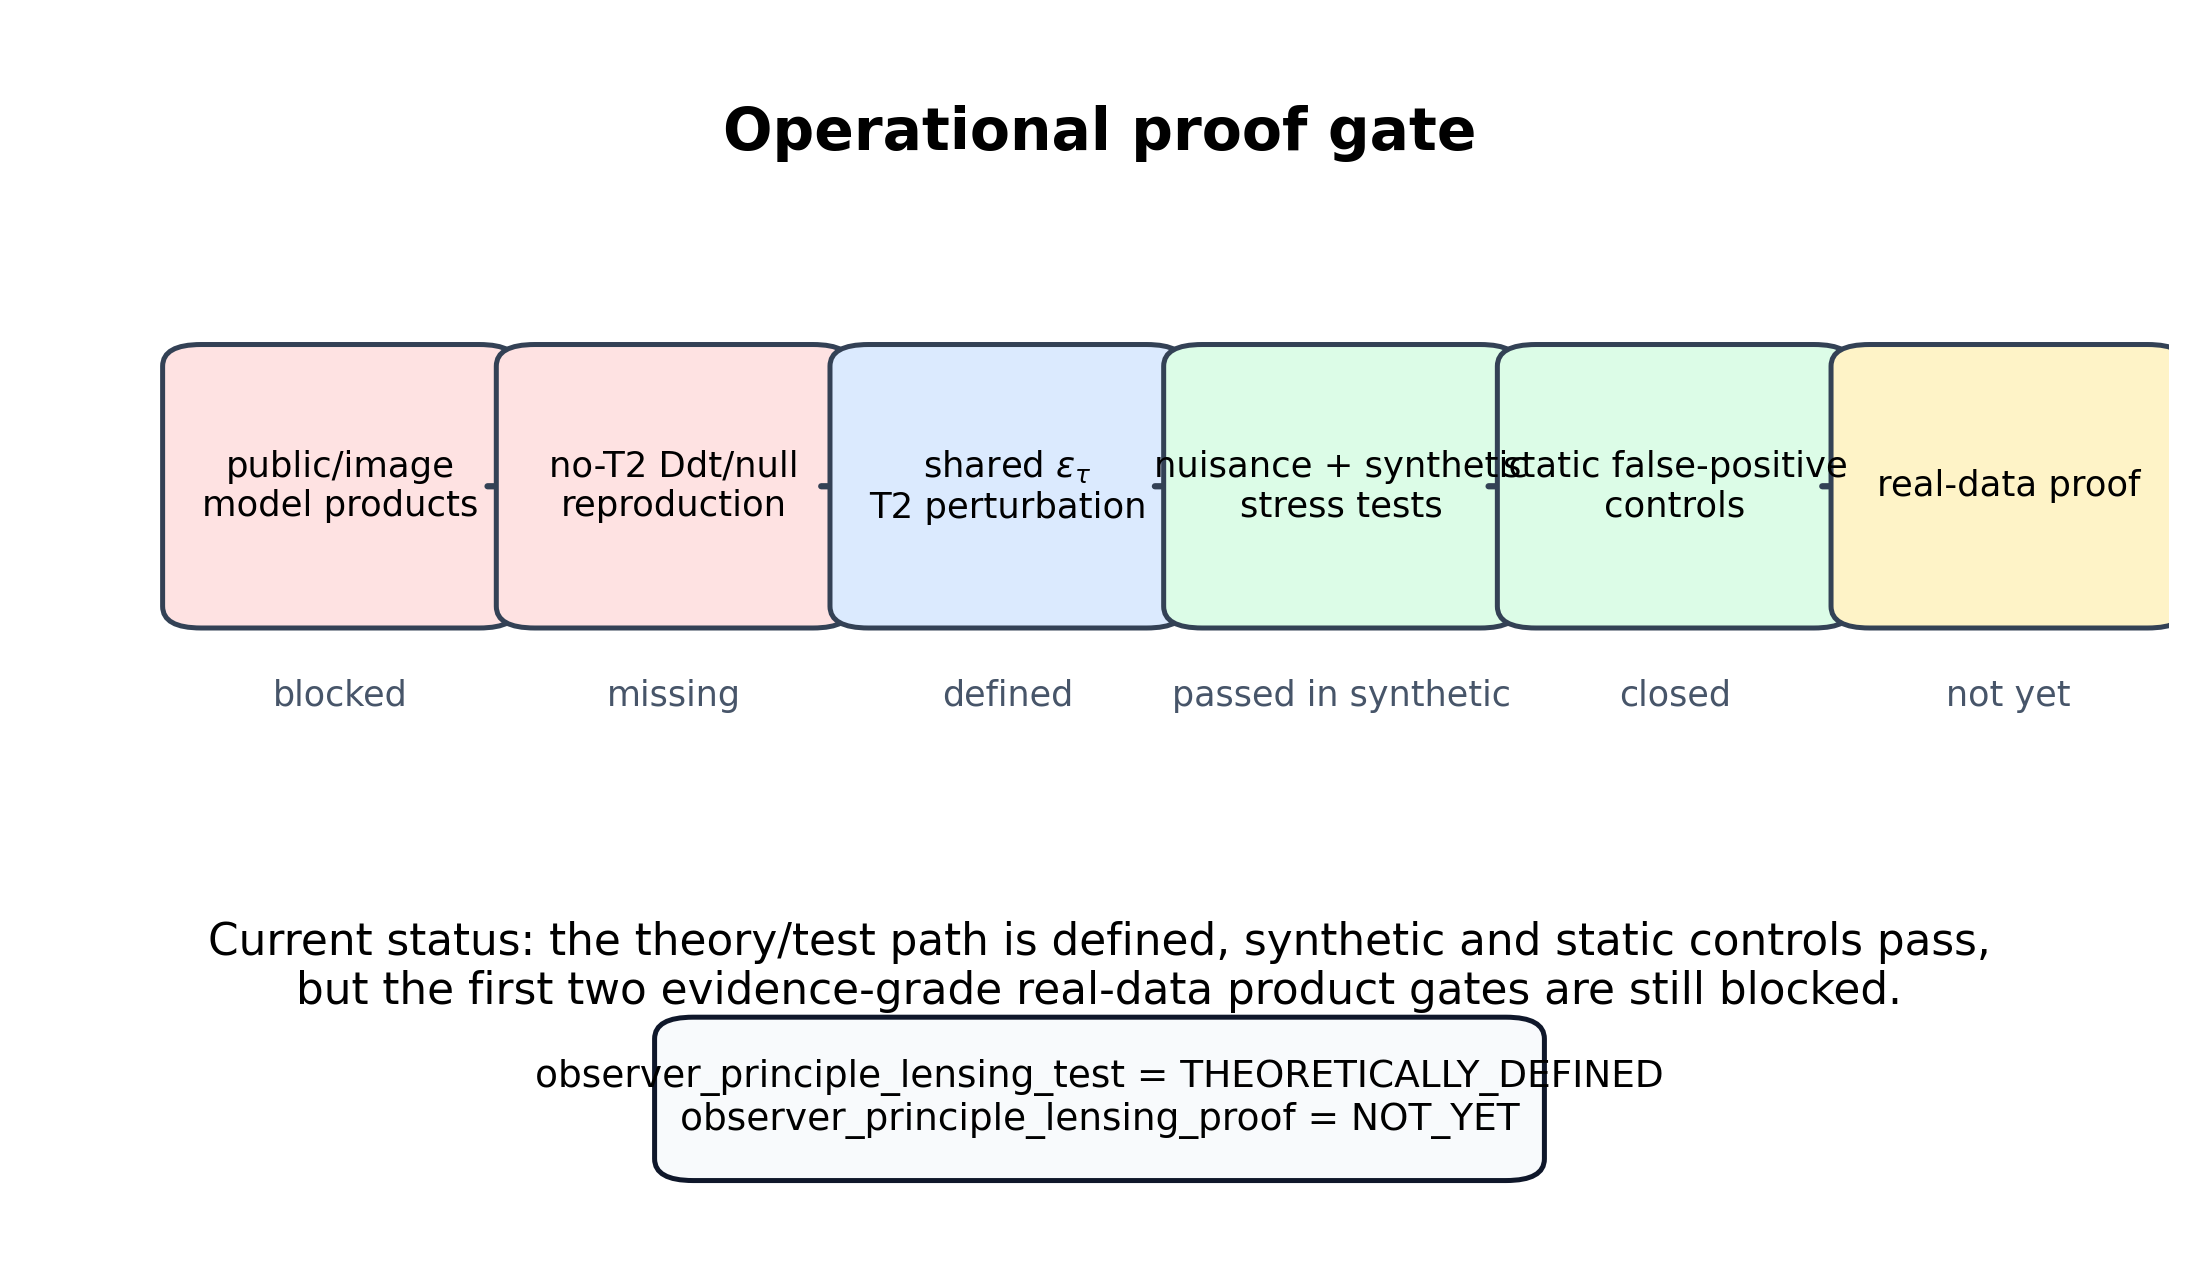
\includegraphics[keepaspectratio,alt={Figure 3. Operational proof gate. The T2 perturbation is not allowed until an evidence-grade no-T2 Ddt/null reproduction is available. Current work defines the test and validates synthetic/static controls, while the first two real-data product gates remain blocked.}]{figures/fig02_proof_gate_flow.png}}
\caption{Figure 3. Operational proof gate. The T2 perturbation is not
allowed until an evidence-grade no-T2 Ddt/null reproduction is
available. Current work defines the test and validates synthetic/static
controls, while the first two real-data product gates remain blocked.}
\end{figure}

\subsection{17. Why Distance Posteriors Alone Are
Insufficient}\label{why-distance-posteriors-alone-are-insufficient}

Published time-delay distance products are valuable cosmography
products, but they are too compressed for the observer-gated T2 proof. A
Ddt posterior alone does not expose which image parity, Fermat-potential
difference, and image-position constraints produced it. Since the T2
channel is image-geometry dependent, the proof must begin upstream of
compressed distance chains.

The required product is therefore not merely:

\begin{Shaded}
\begin{Highlighting}[]
\NormalTok{published Ddt posterior}
\end{Highlighting}
\end{Shaded}

but rather:

\begin{Shaded}
\begin{Highlighting}[]
\NormalTok{image/model products {-}\textgreater{} no{-}T2 Ddt reproduction {-}\textgreater{} controlled T2 perturbation}
\end{Highlighting}
\end{Shaded}

This distinction is the main practical reason the real-data branch is
blocked.

\subsection{18. Synthetic Identifiability
Result}\label{synthetic-identifiability-result}

The synthetic branch asks whether the proposed T2 channel is
mathematically identifiable before any real-data claim is attempted. The
promoted synthetic term was:

\begin{Shaded}
\begin{Highlighting}[]
\NormalTok{T2\_parity\_abs\_fermat}
\end{Highlighting}
\end{Shaded}

It was promoted only after numerical recovery tests and nearby synthetic
controls indicated that it was distinguishable from simpler Fermat-like
alternatives.

Nearby controls did not receive the same status:

{\def\LTcaptype{none} % do not increment counter
\begin{longtable}[]{@{}
  >{\raggedright\arraybackslash}p{(\linewidth - 4\tabcolsep) * \real{0.3333}}
  >{\raggedright\arraybackslash}p{(\linewidth - 4\tabcolsep) * \real{0.3333}}
  >{\raggedright\arraybackslash}p{(\linewidth - 4\tabcolsep) * \real{0.3333}}@{}}
\toprule\noalign{}
\begin{minipage}[b]{\linewidth}\raggedright
Term
\end{minipage} & \begin{minipage}[b]{\linewidth}\raggedright
Role
\end{minipage} & \begin{minipage}[b]{\linewidth}\raggedright
Status
\end{minipage} \\
\midrule\noalign{}
\endhead
\bottomrule\noalign{}
\endlastfoot
\texttt{T1\_fermat} & ordinary Fermat-like control & expected control
fail \\
\texttt{T2}: parity-weighted absolute Fermat & active tau-core branch &
promoted in synthetic tests \\
\texttt{T3}: path-weighted proxy & proxy branch & not promoted as
physics claim \\
\end{longtable}
}

The main hierarchical synthetic result was:

\begin{Shaded}
\begin{Highlighting}[]
\NormalTok{lens\_count = 28}
\NormalTok{position\_constraint\_rows = 224}
\NormalTok{injected epsilon\_tau = 0.05}
\NormalTok{epsilon\_hat = 0.0499193089}
\NormalTok{epsilon\_error = {-}0.0000806911}
\end{Highlighting}
\end{Shaded}

Additional synthetic stress results:

\begin{Shaded}
\begin{Highlighting}[]
\NormalTok{blind\_challenge\_scenarios = 4}
\NormalTok{strict\_identified\_count = 4}
\NormalTok{max\_abs\_epsilon\_error = 0.0003890250}
\end{Highlighting}
\end{Shaded}

Noise Monte Carlo:

\begin{Shaded}
\begin{Highlighting}[]
\NormalTok{replicates\_per\_noise = 64}
\NormalTok{stable\_noise\_max = 0.008}
\NormalTok{transition\_noise\_min = 0.010}
\NormalTok{fail\_noise\_min = null}
\end{Highlighting}
\end{Shaded}

Joint stress grid:

\begin{Shaded}
\begin{Highlighting}[]
\NormalTok{scenario\_count = 8}
\NormalTok{replicates\_per\_scenario = 48}
\NormalTok{stable\_count = 6}
\NormalTok{transition\_count = 2}
\NormalTok{fail\_count = 0}
\end{Highlighting}
\end{Shaded}

Interpretation: the synthetic recovery is a generative sanity check, not
evidence for new physics. Recovering an injected \(\epsilon_\tau=0.05\)
mainly shows that the estimator can recover the signal class it was
asked to recover under controlled assumptions. Its value is
methodological: it checks identifiability, code behavior, stress
degradation, and nearby-control behavior before any real-data claim is
attempted. It does not show that nature contains the T2 operator.

\begin{figure}
\centering
\pandocbounded{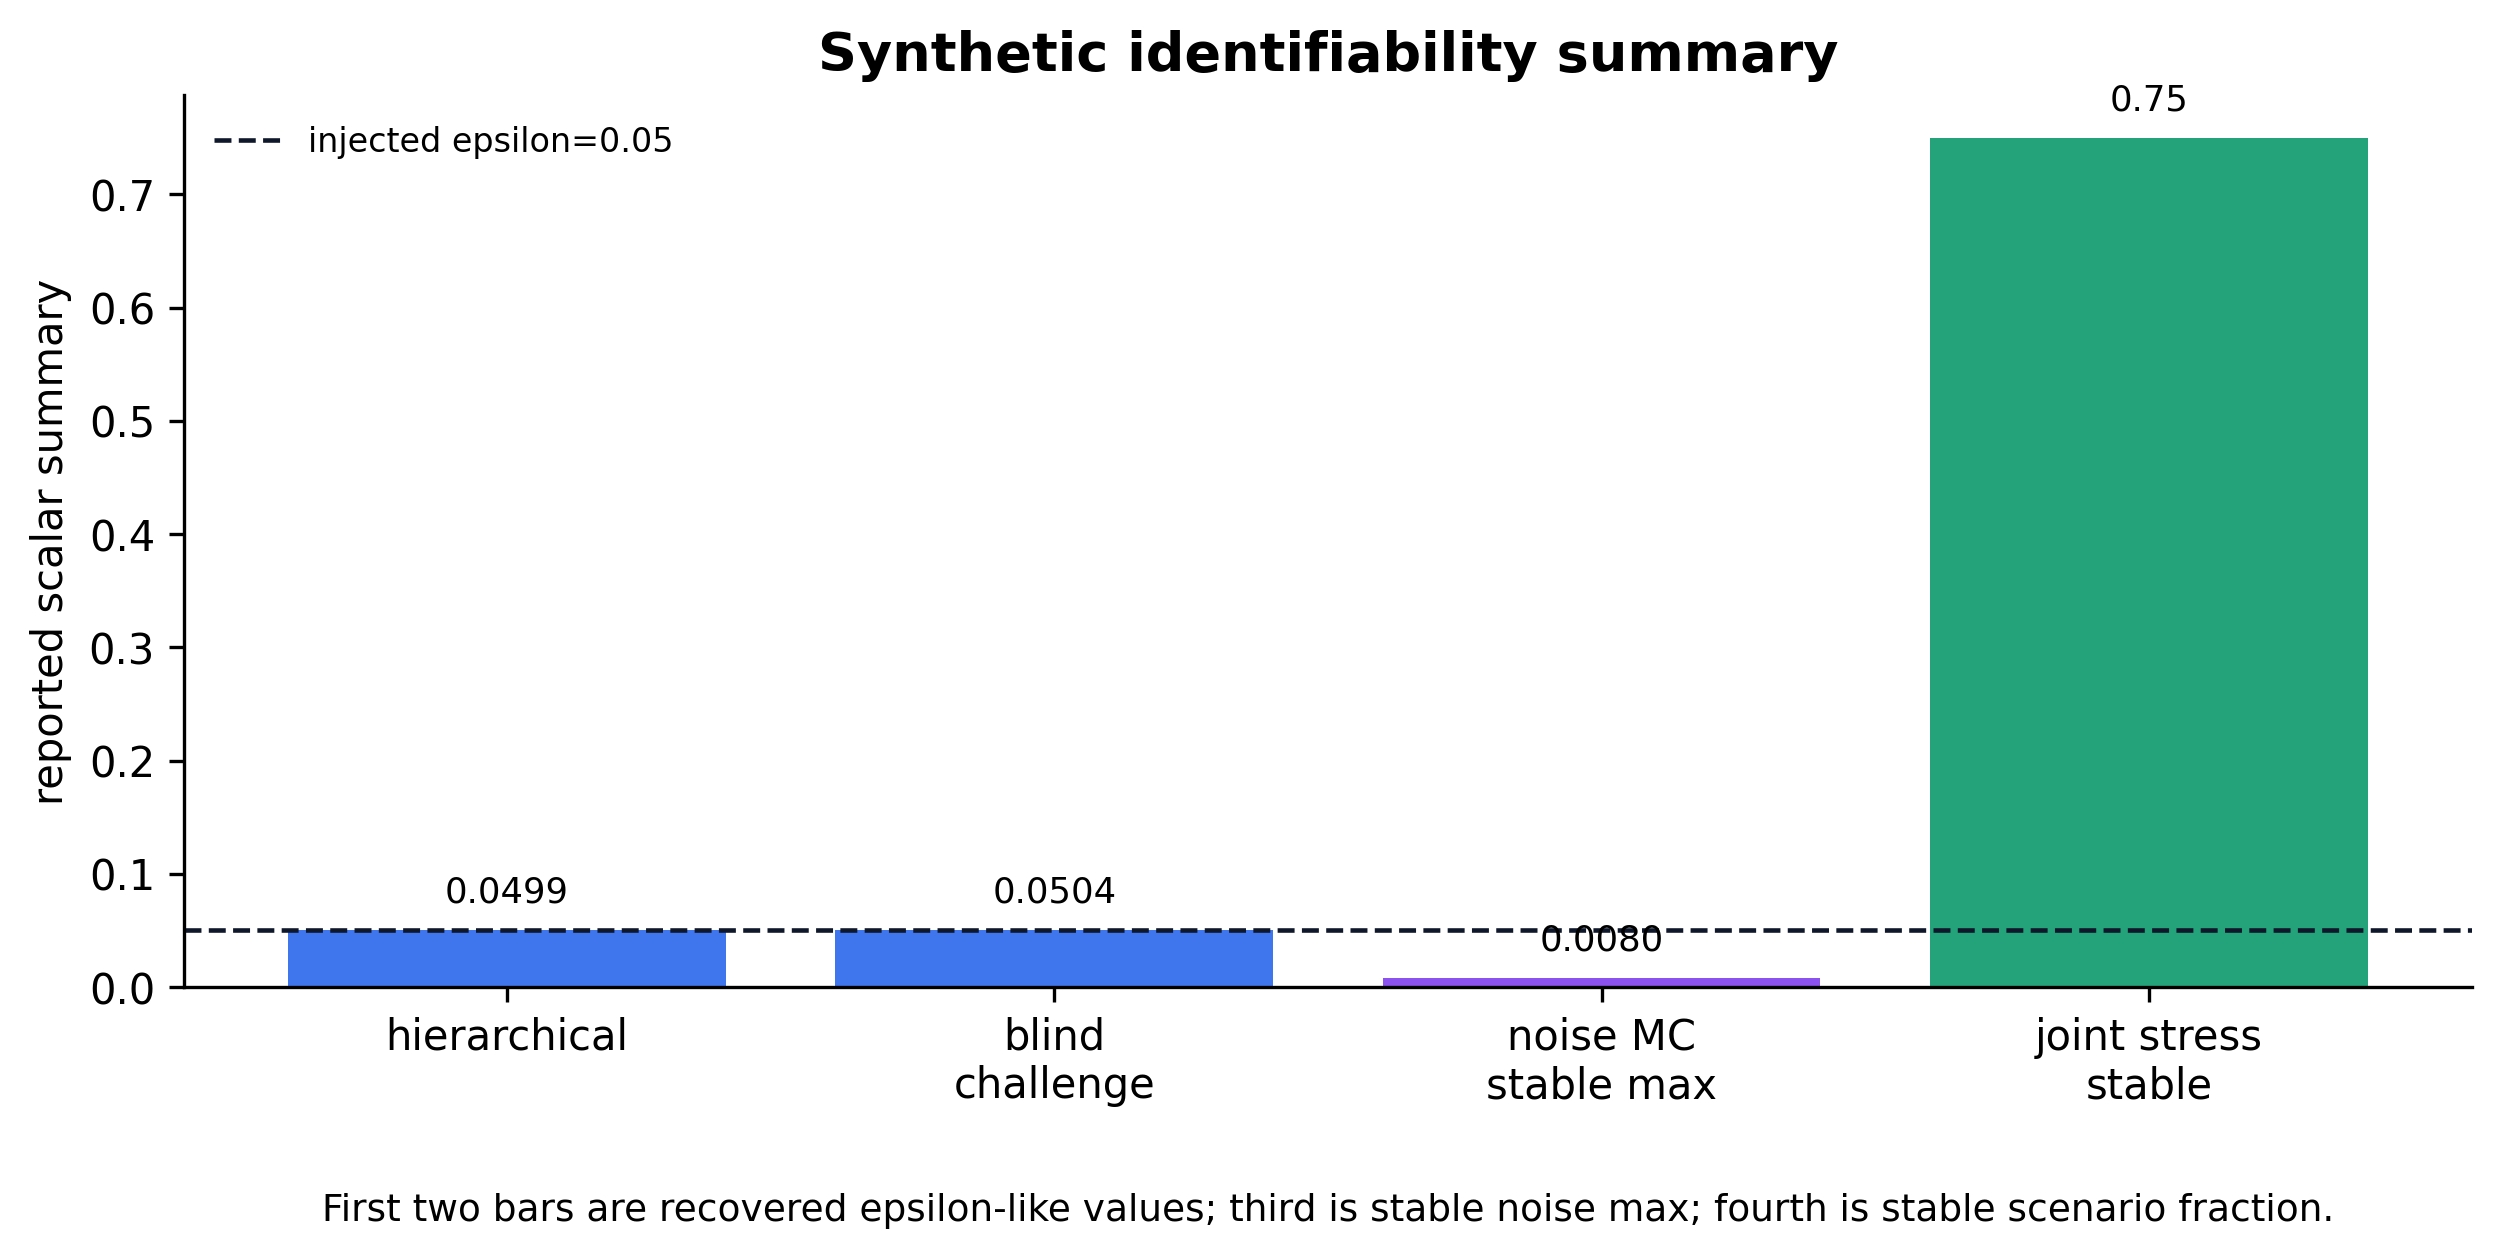
\includegraphics[keepaspectratio,alt={Figure 4. Synthetic identifiability summary. The recovered synthetic epsilon-like values remain near the injected amplitude, while cached stress tests map where stability begins to degrade.}]{figures/fig05_synthetic_identifiability_summary.png}}
\caption{Figure 4. Synthetic identifiability summary. The recovered
synthetic epsilon-like values remain near the injected amplitude, while
cached stress tests map where stability begins to degrade.}
\end{figure}

\subsection{19. Public Time-Delay Product
Audit}\label{public-time-delay-product-audit}

The public audit asked whether the required proof gate can be run
without private communication or unpublished products. The answer was
no: the reviewed public products did not provide the target-specific
posterior/configuration and Fermat/parity releases needed for this test.

The blocker is:

\begin{Shaded}
\begin{Highlighting}[]
\NormalTok{public products are compressed, paper{-}only, or software{-}only rather than}
\NormalTok{target{-}specific posterior/configuration and Fermat/parity releases}
\end{Highlighting}
\end{Shaded}

\begin{figure}
\centering
\pandocbounded{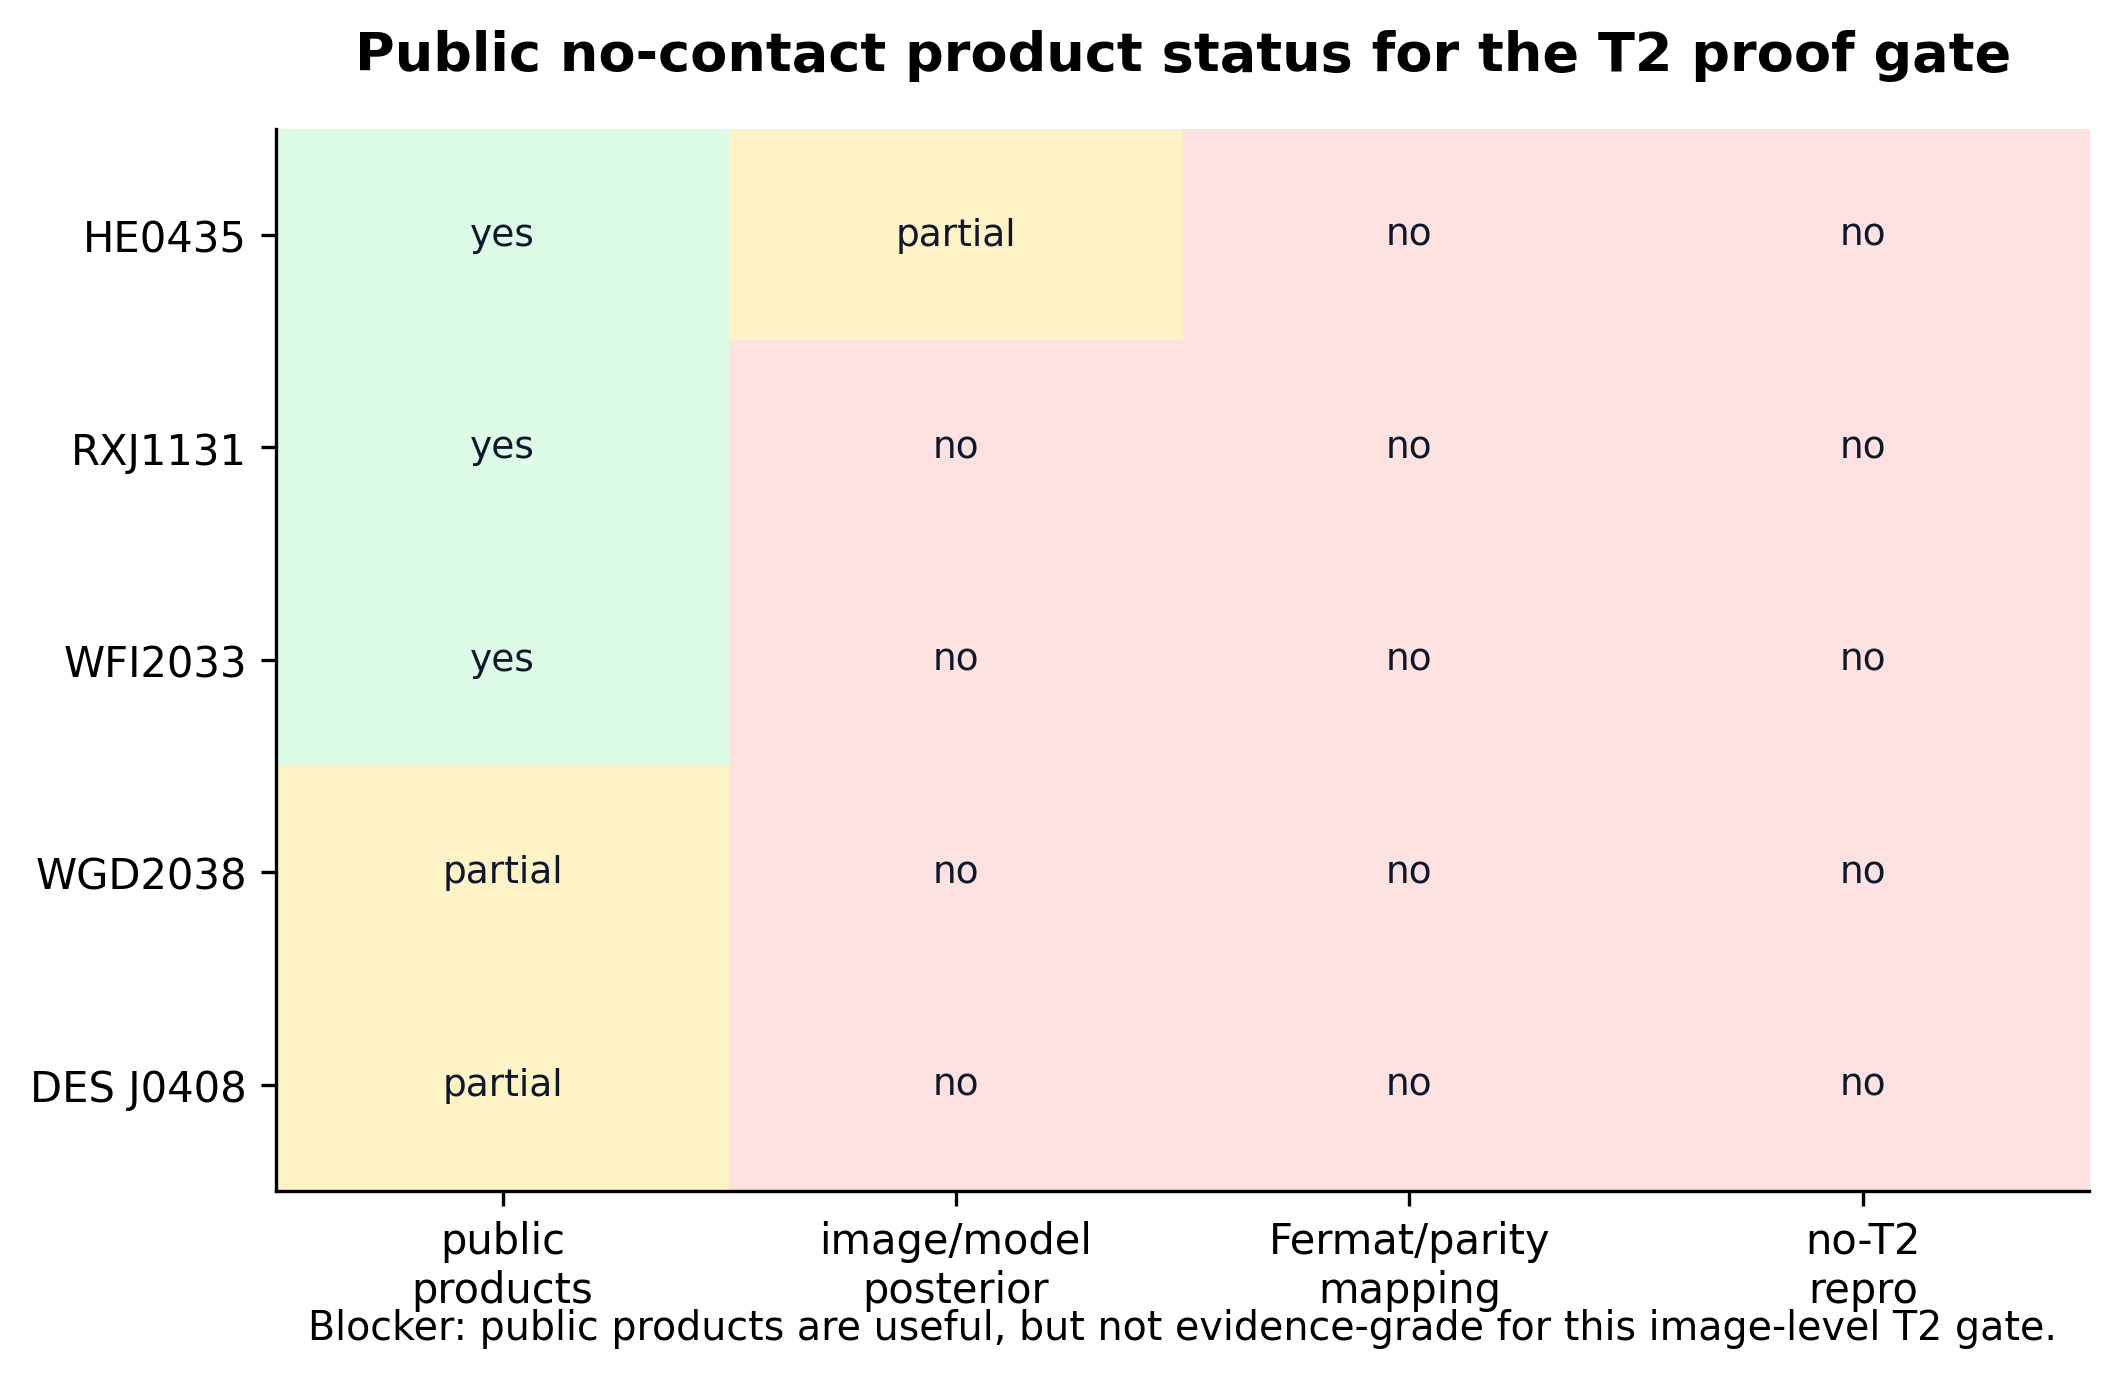
\includegraphics[keepaspectratio,alt={Figure 5. Public no-contact product status for the T2 proof gate. The reviewed targets have useful public products, but not the target-specific image/model posterior and Fermat/parity mapping needed for the no-T2 reproduction gate.}]{figures/fig03_public_product_status_matrix.png}}
\caption{Figure 5. Public no-contact product status for the T2 proof
gate. The reviewed targets have useful public products, but not the
target-specific image/model posterior and Fermat/parity mapping needed
for the no-T2 reproduction gate.}
\end{figure}

\subsubsection{19.1 HE0435-1223}\label{he0435-1223}

HE0435-1223 was the most developed public fallback. Public HST imaging
can be ingested, and the reproduction stack defined Ddt tolerance, label
conventions, pixel masks, null-model requirements, PSF policy, and
archive protocol.

The extracted Ddt tolerance was:

\begin{Shaded}
\begin{Highlighting}[]
\NormalTok{q16/q50/q84 = 2539.56384848 / 2707.4290739999997 / 2889.194643}
\NormalTok{median tolerance = 54.14858148}
\end{Highlighting}
\end{Shaded}

However, the public-only model-level PSF correction attempt did not
reach an evidence-grade reconstruction:

\begin{Shaded}
\begin{Highlighting}[]
\NormalTok{selected\_hard\_bound\_solution\_count = 6}
\NormalTok{baseline\_grid\_ring\_median\_rms = 14.4715078608}
\NormalTok{selected\_ring\_median\_rms = 14.4505423335}
\NormalTok{improvement\_vs\_baseline = 0.0209655273}
\NormalTok{max\_ring\_five\_sigma\_fraction = 0.2173664667}
\end{Highlighting}
\end{Shaded}

This is not a criticism of the published HE0435 analysis. It says only
that our public-only reconstruction is not evidence-grade enough to
support a tau-core perturbation.

\subsubsection{19.2 Other Targets}\label{other-targets}

RXJ1131-1231 and WFI2033-4723 were found to have useful public material,
but the available products were too compressed for the image-level T2
reproduction required here. WGD2038-4008 and DES J0408-5354 were
similarly limited by paper-level or non-target-specific products for
this particular test.

These targets remain scientifically valuable. They are blocked only for
this specific observer-gated proof gate because the required image/model
product depth was not confirmed.

\subsection{20. Static-Lens Controls}\label{static-lens-controls}

Because real time-delay proof products were unavailable, we developed a
static control analysis to test false-positive behavior. The branch used
HFF cluster morphology controls: Chandra gas, HFF lensing mass maps, and
public member-catalog tracers.

The analysis completed five control layers:

{\def\LTcaptype{none} % do not increment counter
\begin{longtable}[]{@{}
  >{\raggedright\arraybackslash}p{(\linewidth - 4\tabcolsep) * \real{0.3333}}
  >{\raggedright\arraybackslash}p{(\linewidth - 4\tabcolsep) * \real{0.3333}}
  >{\raggedright\arraybackslash}p{(\linewidth - 4\tabcolsep) * \real{0.3333}}@{}}
\toprule\noalign{}
\begin{minipage}[b]{\linewidth}\raggedright
Control layer
\end{minipage} & \begin{minipage}[b]{\linewidth}\raggedright
Role
\end{minipage} & \begin{minipage}[b]{\linewidth}\raggedright
\end{minipage} \\
\midrule\noalign{}
\endhead
\bottomrule\noalign{}
\endlastfoot
HFF morphology selection & select an independent static-lens morphology
layer & \\
control scorecard & require heterogeneous controls & \\
null injection & test zero-T2 false positives & \\
null stress sweep & bracket the noise/threshold boundary & \\
systematic-template sweep & flag dangerous templates & \\
\end{longtable}
}

The scorecard was heterogeneous:

\begin{Shaded}
\begin{Highlighting}[]
\NormalTok{strong\_control = 1}
\NormalTok{mixed\_control = 2}
\NormalTok{weak\_negative\_control = 1}
\NormalTok{selected\_static\_control = macs0717}
\NormalTok{selected\_negative\_control = abells1063}
\end{Highlighting}
\end{Shaded}

Baseline null injection:

\begin{Shaded}
\begin{Highlighting}[]
\NormalTok{injected\_epsilon\_tau = 0.0}
\NormalTok{observed\_null\_epsilon\_hat = 0.004678323836468474}
\NormalTok{false\_positive\_rate = 0.0}
\NormalTok{replicates = 2048}
\end{Highlighting}
\end{Shaded}

Stress boundary:

\begin{Shaded}
\begin{Highlighting}[]
\NormalTok{reference\_threshold = 0.05}
\NormalTok{reference\_threshold\_stable\_max\_noise = 0.020}
\NormalTok{first transition at threshold 0.05: noise\_sigma = 0.030}
\end{Highlighting}
\end{Shaded}

Template sensitivity:

\begin{Shaded}
\begin{Highlighting}[]
\NormalTok{nominal\_templates\_all\_stable = true}
\NormalTok{inverted\_morphology: transition, false\_positive\_rate = 0.010498046875}
\NormalTok{residual\_aligned\_adversarial: fails, false\_positive\_rate = 0.70947265625}
\end{Highlighting}
\end{Shaded}

The static controls support the falsification discipline of the proof
program: the workflow does not automatically see tau-core structure
everywhere. But static controls contain no time-delay posterior and
therefore cannot prove the observer principle.

\begin{figure}
\centering
\pandocbounded{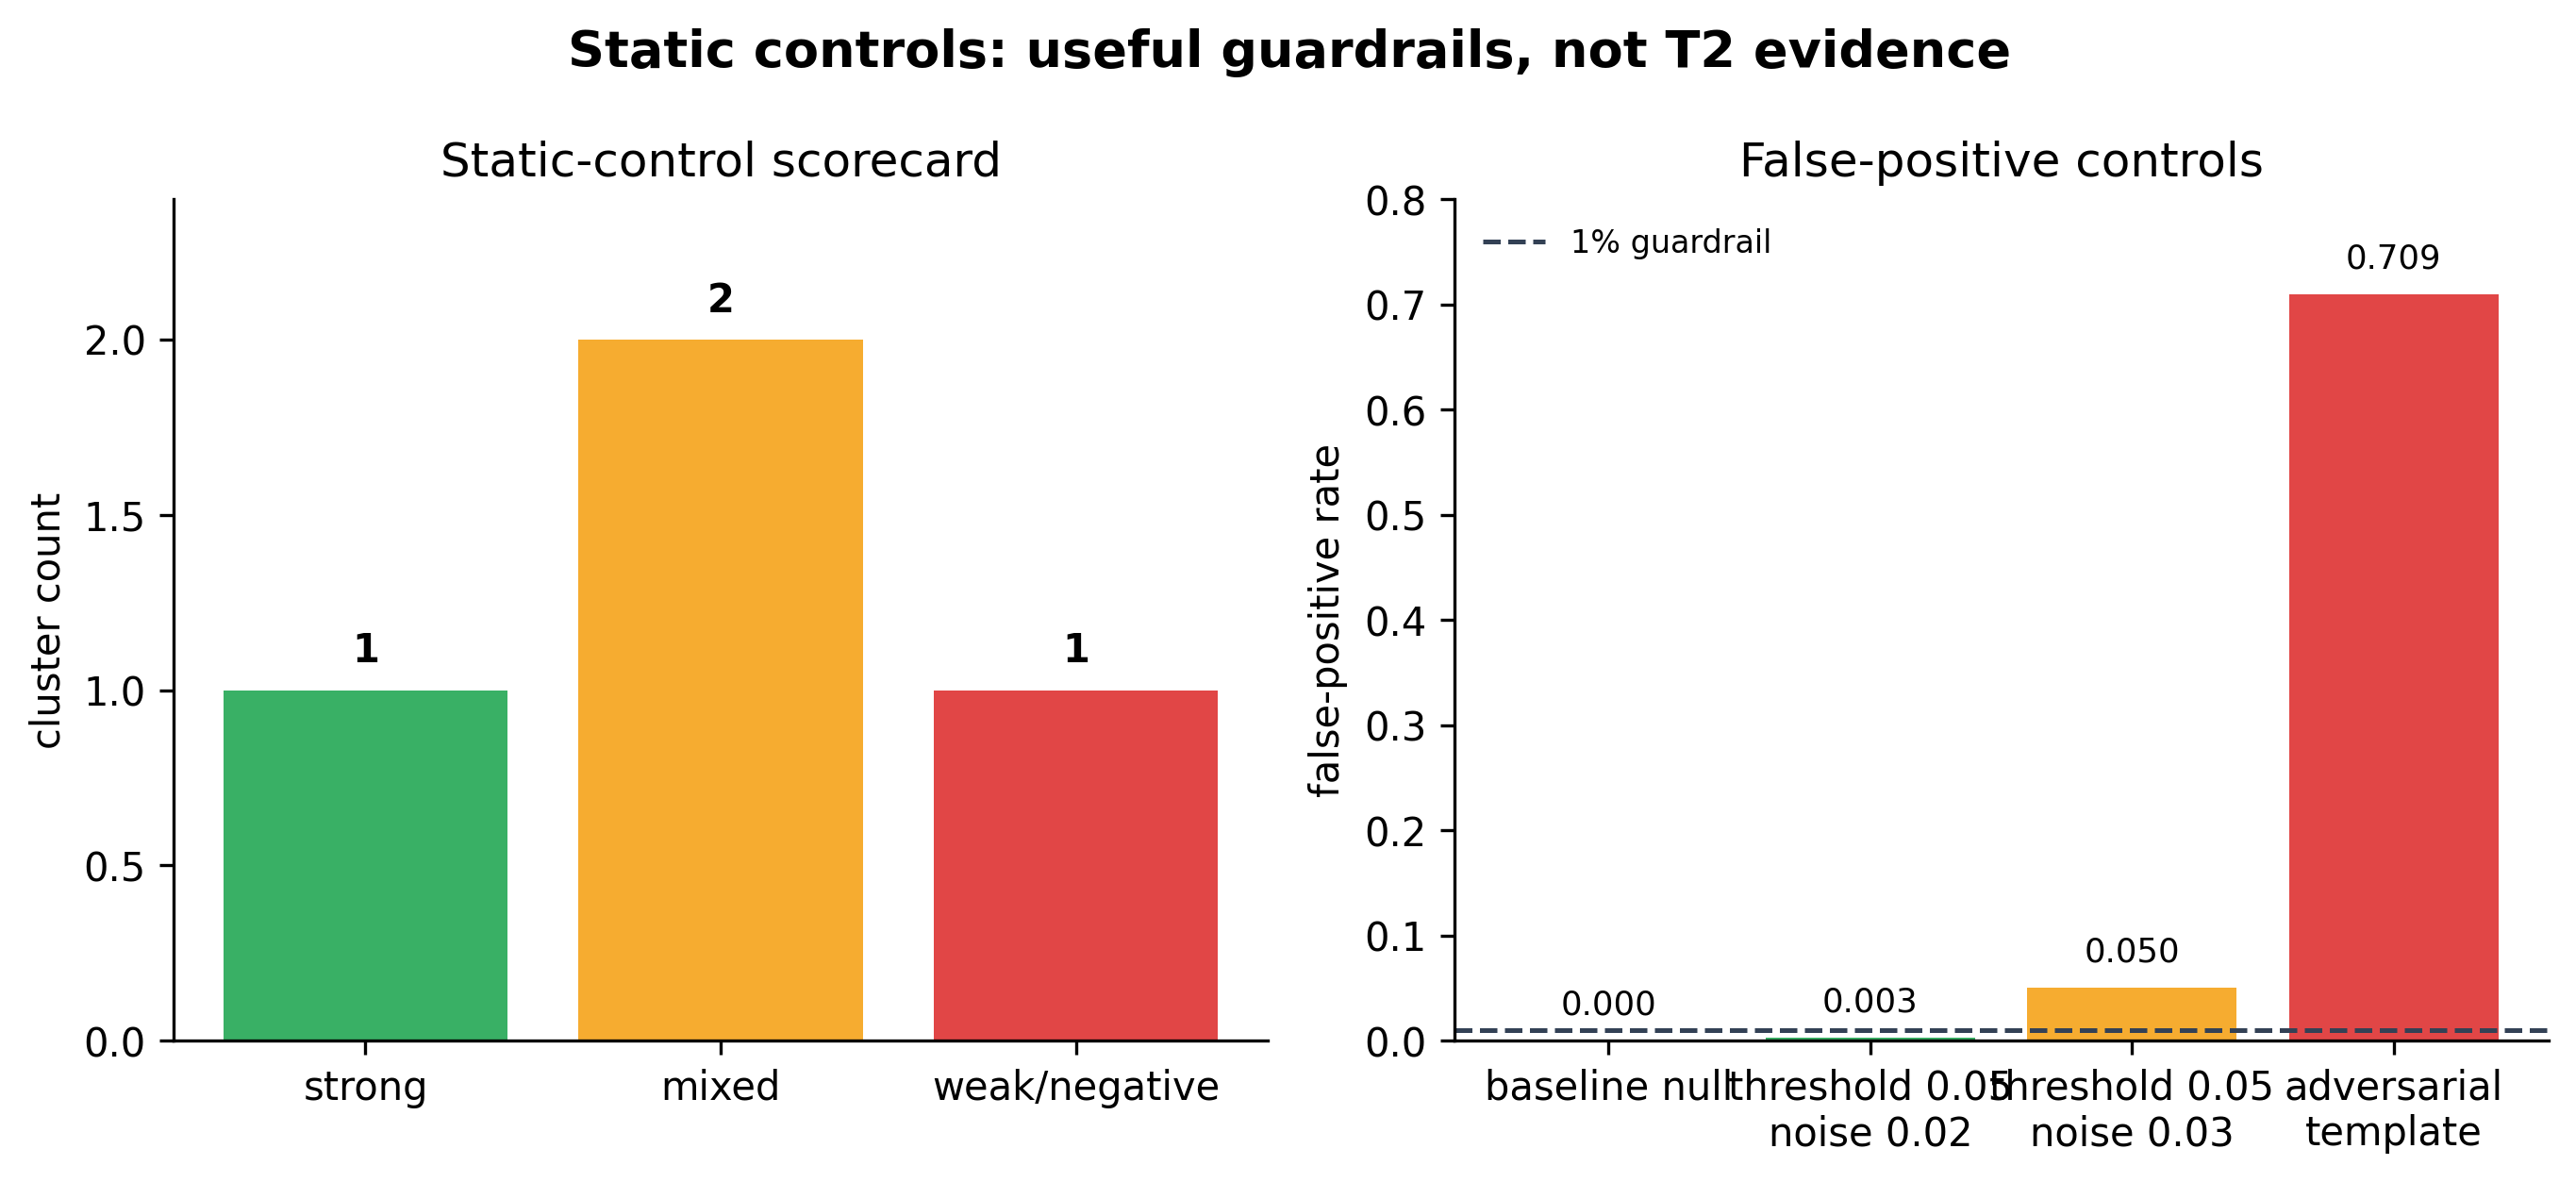
\includegraphics[keepaspectratio,alt={Figure 6. Static-control guardrails. HFF morphology controls remain heterogeneous, pass the baseline null-injection test, and expose noise/template regimes where false positives can be manufactured.}]{figures/fig04_static_control_guardrails.png}}
\caption{Figure 6. Static-control guardrails. HFF morphology controls
remain heterogeneous, pass the baseline null-injection test, and expose
noise/template regimes where false positives can be manufactured.}
\end{figure}

\subsection{21. Anticipated Reviewer
Objections}\label{anticipated-reviewer-objections}

The most likely reviewer objections are valid, and the paper should be
read with them in view.

{\def\LTcaptype{none} % do not increment counter
\begin{longtable}[]{@{}
  >{\raggedright\arraybackslash}p{(\linewidth - 2\tabcolsep) * \real{0.5000}}
  >{\raggedright\arraybackslash}p{(\linewidth - 2\tabcolsep) * \real{0.5000}}@{}}
\toprule\noalign{}
\begin{minipage}[b]{\linewidth}\raggedright
Objection
\end{minipage} & \begin{minipage}[b]{\linewidth}\raggedright
Correct response in this paper
\end{minipage} \\
\midrule\noalign{}
\endhead
\bottomrule\noalign{}
\endlastfoot
The T2 operator looks handcrafted. & Partly. The manuscript now gives a
conditional weak-field route, but T2 is still not a derived necessity
until the assumptions are obtained from an action, reciprocity theorem,
or covariant observer construction. \\
The synthetic recovery is too clean. & Yes. It is a sanity check showing
recovery from a known generative class, not evidence that the class is
realized in nature. \\
There is no real-data posterior. & Correct. No no-T2 Ddt/null
reproduction, real-data Bayes factor, or posterior-predictive check is
claimed. \\
The tau-core background theory is too open. & Correct. The paper does
not yet specify what fundamental object transforms, what is invariant,
or what the primitive measurable is in a complete theory. \\
The axioms are imposed, not derived. & Correct. The paper now maps their
possible origins, but path-reversal evenness, Morse-orientation
coupling, and covariant closure remain open theory tasks. \\
The reciprocity principle is missing. & Partly. The thin-lens
reciprocity lemma is proven, but no full covariant reciprocity theorem
is claimed. \\
There is no covariant measurable. & Partly. The paper now proposes an
optical measurable candidate using observer proper-time depth and
Jacobi-map orientation, but it is not yet derived from a full tau-core
action. \\
The shared amplitude is imposed. & Partly. The paper now gives a
tau-accessibility current candidate, but no conservation theorem has yet
been proven. \\
The current has no action origin. & Partly. The paper gives a minimal
Noether-current route from tau shift symmetry, but no complete covariant
action is claimed. \\
The screen construction may be gauge-dependent. & Partly. The paper
states screen-gauge covariance conditions, but a full action-level
derivation is still missing. \\
There is no dynamical closure. & Correct. The paper now states the
required stress-energy, conservation, and GR-limit conditions, but does
not derive them from a complete action. \\
\end{longtable}
}

These objections do not invalidate the narrower contribution. They
define its scope. The present manuscript is best classified as a methods
and feasibility note with a physics kernel, not as a new-physics
detection paper.

\subsection{22. Main Proposition of the
Paper}\label{main-proposition-of-the-paper}

We can now state the paper's central theorem in operational form.

\textbf{Proposition.} An operational gravitational-lensing test of the
tau-core observer principle is theoretically possible because the
observer principle can be mapped to an image-level time-delay lensing
operator family with a shared population-level amplitude. The present
candidate operator is \texttt{T2\_parity\_abs\_fermat}. This proposition
does not assert that a complete tau-core action, field content,
covariance structure, conservation law, GR-limit derivation, gauge
interpretation, or operator-selection principle has been supplied. A
future empirical proof would require the T2 amplitude to be identified
only after a no-T2 Ddt/null reproduction, likelihood-level nuisance
marginalization, evidence comparison against nearby operators, and
synthetic and static false-positive controls.

\textbf{Status.} The present work verifies the synthetic and control
components of this theorem, but not the real-data no-T2 reproduction
component.

Therefore:

\begin{Shaded}
\begin{Highlighting}[]
\NormalTok{tau{-}lensing perturbation test: defined at phenomenological Level 1}
\NormalTok{real{-}data proof: not yet achieved}
\NormalTok{complete tau{-}core field theory: not yet supplied}
\NormalTok{dynamical operator{-}selection principle: not yet supplied}
\NormalTok{geometrical necessity theorem: not yet supplied}
\NormalTok{missing ingredient: evidence{-}grade time{-}delay image/model products}
\end{Highlighting}
\end{Shaded}

This is the strongest defensible conclusion.

\subsection{23. Data Used and
Reproducibility}\label{data-used-and-reproducibility}

The present work used three categories of material.

First, public time-delay lensing product information was audited through
local source manifests and product probes. This included HE0435-1223,
RXJ1131-1231, WFI2033-4723, WGD2038-4008, DES J0408-5354, H0LiCOW public
distance products, TDCOSMO public notebook routes, and related public
repositories or metadata pages. These products were sufficient to define
blockers but not sufficient to authorize the no-T2 reproduction gate.

Second, synthetic lensing data were used to test whether the proposed T2
channel is identifiable in principle. These tests do not use real
lensing measurements as evidence; they test the mathematical behavior of
the proposed estimator under controlled noise, nuisance, and
position-constraint assumptions.

Third, static HFF cluster products were used as false-positive controls.
These include already-generated summaries from Chandra gas, HFF lensing
mass maps, and member-catalog morphology controls. They test whether the
workflow becomes over-eager in systems without time-delay evidence.

Primary packet:

Primary packet:

\begin{Shaded}
\begin{Highlighting}[]
\NormalTok{studies/tau\_core\_lensing\_observer\_gate\_v01/paper\_packet\_v01\_public\_blocked/}
\end{Highlighting}
\end{Shaded}

Critical scripts:

\begin{Shaded}
\begin{Highlighting}[]
\NormalTok{repro/scripts/check\_repro.py}
\NormalTok{repro/scripts/build\_pdfs.py}
\NormalTok{studies/tau\_core\_lensing\_observer\_gate\_v01/make\_manuscript\_pdf.py}
\NormalTok{studies/tau\_core\_lensing\_observer\_gate\_v01/make\_arxiv\_source.py}
\end{Highlighting}
\end{Shaded}

Critical outputs:

\begin{Shaded}
\begin{Highlighting}[]
\NormalTok{outputs/tau\_core\_lensing\_observer\_gate\_v01/}
\NormalTok{repro/results/*/summary.json}
\end{Highlighting}
\end{Shaded}

Run:

\begin{Shaded}
\begin{Highlighting}[]
\ExtensionTok{python}\NormalTok{ repro/scripts/check\_repro.py}
\ExtensionTok{python}\NormalTok{ studies/tau\_core\_lensing\_observer\_gate\_v01/make\_manuscript\_pdf.py}
\ExtensionTok{python}\NormalTok{ studies/tau\_core\_lensing\_observer\_gate\_v01/make\_arxiv\_source.py}
\ExtensionTok{python} \AttributeTok{{-}m}\NormalTok{ pytest }\AttributeTok{{-}q}
\end{Highlighting}
\end{Shaded}

Expected:

\begin{Shaded}
\begin{Highlighting}[]
\NormalTok{REPRO\_CHECK\_PASS}
\NormalTok{4 passed}
\end{Highlighting}
\end{Shaded}

\subsection{24. Limitations}\label{limitations}

\begin{enumerate}
\def\labelenumi{\arabic{enumi}.}
\tightlist
\item
  No real-data T2 posterior was sampled.
\item
  No public-only target passed the no-T2 Ddt/null reproduction gate.
\item
  The HE0435 public fallback failed PSF/model validation and is not a
  published-posterior reproduction.
\item
  Synthetic tests validate method behavior, not astrophysical truth.
\item
  Static controls are false-positive controls, not time-delay evidence.
\item
  The contact route for original products was disabled by user choice in
  this work session.
\item
  The tau-core observer principle is not yet a closed physical theory:
  action, field content, covariance structure, symmetry, conservation
  relation, first-principles GR limit, and gauge meaning remain open.
\item
  The T2 operator is not yet dynamically derived. The paper gives a
  conditional weak-field route, but its assumptions remain to be derived
  from a deeper theory and it must be tested against a predefined
  operator family.
\item
  No real-data likelihood, evidence, Bayes factor, prior-sensitivity
  analysis, or posterior-predictive check has yet been computed.
\item
  No geometrical necessity theorem, reciprocity theorem, variational
  derivation, or symmetry selection rule has yet been supplied for T2.
\item
  The paper has not yet defined the primitive physical measurable of
  \texttt{tau(x;\ u)} in a complete theory: what transforms, what
  remains invariant, and what detector-accessible quantity carries the
  tau-core correction.
\item
  The theorem attempt depends on axioms whose origins are only partially
  identified; path-reversal evenness, Morse-orientation coupling,
  conserved tau current, and covariant closure remain open.
\item
  The reciprocity principle is proven only as a thin-lens lemma. A
  covariant theorem deriving the measurable, the reversal map, and the
  current structure has not yet been supplied.
\item
  No covariant detector-accessible tau-core measurable has yet been
  derived; the paper lists candidates but does not prove their
  invariance or thin-lens reduction.
\item
  The optical measurable
  \(\mathcal{O}_{\tau,i}^\mathrm{cov}=\Sigma_i\mathcal{P}(T_i^\mathrm{cov})\)
  is a candidate reduction, not yet a consequence of a full action or
  conserved tau current.
\item
  The tau-accessibility current \(J^\mu_\tau\) is only a closure
  candidate; no conservation theorem has yet been derived that forces a
  shared \(\epsilon_\tau\).
\item
  The Noether-current route assumes a tau shift symmetry and a screen
  interaction term; neither has yet been derived from a complete
  covariant tau-core action.
\item
  Screen-gauge covariance is specified only as a consistency condition;
  the distinction between physical orientation reversal and arbitrary
  screen relabeling remains to be derived from a complete observer
  construction.
\item
  Dynamical closure is not derived: the stress-energy contribution,
  conservation relation, screen response, and GR limit remain
  requirements for a future complete theory.
\end{enumerate}

\subsection{25. Conclusion}\label{conclusion}

Gravitational lensing provides a natural route toward testing the
tau-core observer principle because a single lens supplies multiple
observer-accessible image channels. This paper formulates the required
proof criterion and identifies \texttt{T2\_parity\_abs\_fermat} as the
operative synthetic channel. The channel is identifiable in controlled
synthetic tests and is protected by static false-positive controls.

The proof is not yet complete, and the underlying tau-core theory is not
yet complete either. The physics kernel is embryonic: no geometrical
necessity theorem, symmetry selection rule, reciprocity argument, or
variational derivation currently forces T2. Public no-contact products
also do not provide the evidence-grade image/model chain needed to
reproduce a no-T2 Ddt/null posterior. The line is therefore
scientifically alive at the phenomenological test level, but the
real-data claim, the operator-necessity claim, and the full physical
theory claim remain open.

The next decisive step is not another static control. It is an
evidence-grade time-delay lens product chain that permits:

\begin{Shaded}
\begin{Highlighting}[]
\NormalTok{no{-}T2 Ddt/null reproduction {-}\textgreater{} shared{-}epsilon T2 perturbation {-}\textgreater{} nuisance and}
\NormalTok{false{-}positive controls}
\end{Highlighting}
\end{Shaded}

Only that sequence can turn the proof program into an empirical proof.

\subsection{References and Source
Anchors}\label{references-and-source-anchors}

\begin{itemize}
\tightlist
\item
  Suyu et al.~/ H0LiCOW public data products:
  \url{https://shsuyu.github.io/H0LiCOW/site/h0licow_data.html}
\item
  H0LiCOW Paper I overview:
  \url{https://academic.oup.com/mnras/article/468/3/2590/3055701}
\item
  TDCOSMO I public notebook path:
  \url{https://github.com/TDCOSMO/TD_data_public/blob/master/TDCOSMO_I/PSTD_notebook.ipynb}
\item
  TDCOSMO I time-delay cosmography methods PDF:
  \url{https://lss.fnal.gov/archive/2019/pub/fermilab-pub-19-665-scd.pdf}
\item
  TDCOSMO XXVI Zenodo metadata:
  \url{https://zenodo.org/records/19421439}
\item
  Local feasibility ledger: \texttt{feasibility\_ledger.md}
\end{itemize}

\end{document}
